  \documentclass[english,msc,numbers,hidelinks]{coppe}

\usepackage{amsmath,amssymb}
\usepackage{hyperref}
\usepackage{longtable}
\usepackage{booktabs}
\usepackage{float}
% Change to Captions
\usepackage{caption}
\usepackage[font=footnotesize,labelfont={it}]{caption}

\providecommand{\tightlist}{%
  \setlength{\itemsep}{0pt}\setlength{\parskip}{0pt}}

\makelosymbols
\makeloabbreviations


% From {rticles}
\newlength{\csllabelwidth}
\setlength{\csllabelwidth}{3em}
\newlength{\cslhangindent}
\setlength{\cslhangindent}{1.5em}
% for Pandoc 2.8 to 2.10.1
\newenvironment{cslreferences}%
  {}%
  {\par}
% For Pandoc 2.11+
% As noted by @mirh [2] is needed instead of [3] for 2.12
\newenvironment{CSLReferences}[2] % #1 hanging-ident, #2 entry spacing
 {% don't indent paragraphs
  \setlength{\parindent}{0pt}
  % turn on hanging indent if param 1 is 1
  \ifodd #1 \everypar{\setlength{\hangindent}{\cslhangindent}}\ignorespaces\fi
  % set entry spacing
  \ifnum #2 > 0
  \setlength{\parskip}{#2\baselineskip}
  \fi
 }%
 {}
\usepackage{calc} % for calculating minipage widths
\newcommand{\CSLBlock}[1]{#1\hfill\break}
\newcommand{\CSLLeftMargin}[1]{\parbox[t]{\csllabelwidth}{#1}}
\newcommand{\CSLRightInline}[1]{\parbox[t]{\linewidth - \csllabelwidth}{#1}}
\newcommand{\CSLIndent}[1]{\hspace{\cslhangindent}#1}
\begin{document}

  \title{Titulo de Tese}
  \foreigntitle{Thesis' Title}
    \author{Jefferson T.}{Silvério}
      \advisor{Prof.}{Gisele A.}{Oda}{D.Sc.}
    \advisor{Prof.}{Verónica}{Valentinuzzi}{Ph.D}
    \advisor{Prof.}{Patricia}{Tachinardi}{Ph.D}
  

    \examiner{Prof.}{Nome Completo do Primeiro Examinador}{D.Sc.}
    \examiner{Prof.}{Nome Completo do Segundo Examinador}{Ph.D}
    \examiner{Prof.}{Nome Completo do Terceiro Examinador}{Ph.D}
    \department{IB}
  \date{08}{2021}
    \keyword{Primeira palavra-chave}
    \keyword{biologging}
    
  % Adiciona Pagina de Titulo
  \maketitle

  % Adiciona Pagina de Rosto com 
  \frontmatter
  
  %Adiciona dedicatorias
  \dedication{A alguém cujo valor é digno desta dedicatória.}
    \chapter*{Agradecimentos}
  Gostaria de agradecer a X
  
  % Adiciona Abstracts
  \begin{abstract}
  ABSTRACT
  \end{abstract}
  \pagebreak
  \begin{foreignabstract}
  ABSTRACT INGLES
  \end{foreignabstract}
  % Adiciona Sumário
  \tableofcontents
  
  % Adiciona Lista de Figuras
    \listoffigures
  
  % Adiciona Lista de Tabelas
    \listoftables
  
  % Adiciona Lista de Simbolos e Abreviacoes
  \printlosymbols
  \printloabbreviations

  % Adiciona Corpo da Tese
  \mainmatter
  \hypertarget{daily-activity-patterns-in-the-anillaco-tuco-tuco-ctenomys-sp.}{%
  \chapter{\texorpdfstring{Daily activity patterns in the Anillaco Tuco-tuco (\emph{Ctenomys sp.})}{Daily activity patterns in the Anillaco Tuco-tuco (Ctenomys sp.)}}\label{daily-activity-patterns-in-the-anillaco-tuco-tuco-ctenomys-sp.}}

  \hypertarget{introduction}{%
  \section{Introduction}\label{introduction}}
  \begin{itemize}
  \tightlist
  \item
    Contexto:
  \item
    Síntese do conhecimento:O que se sabe sobe o tema central?
  \item
    Como a questão investigada se encaixa nesse contexto teórico?
  \item
    Rever anotações
  \end{itemize}
  \hypertarget{methods}{%
  \section{Methods}\label{methods}}
  \begin{itemize}
  \tightlist
  \item
    Adicionar descrição da estatistica
  \item
    Adicionar Kernel Density Estimation para os padrões
  \end{itemize}
  \hypertarget{study-species}{%
  \subsection{Study Species}\label{study-species}}

  The studied \emph{Ctenomys} population lacks a formal phylogenetic and taxonomic classification but there are some lines of evidence suggesting that the study area is occupied by a single unidentified species (\protect\hyperlink{ref-amaya2016}{Amaya et al. 2016}). In other studies this \emph{Ctenomys'} species has been referred informally as the Anillaco tuco-tuco (\protect\hyperlink{ref-amaya2016}{Amaya et al. 2016}) and as \emph{Ctenomys} aff. \emph{knightii} (\protect\hyperlink{ref-tomotani2012}{Tomotani et al. 2012}) or \emph{Ctenomys} cf.~\emph{knightii} (\protect\hyperlink{ref-valentinuzzi2009}{Valentinuzzi et al. 2009}).

  \hypertarget{study-site}{%
  \subsection{Study Site}\label{study-site}}

  Field work was conducted at a site located approximately 5km away from the village of Anillaco, in the province of La Rioja, northwest of Argentina. The study site (-66.95°, -028.80, 1325m; Fig. \ref{fig:methods-map}) is a relatively undisturbed natural area, with little human disturbance and no artificial light source. The area is surrounded by the Sierra de Velasco moutain range, located within the Monte Desert biome. The Monte Desert is characterized as an open shrubland dominated by Zygophyllaceae (\emph{Larrea cuneifolia} Cav., \emph{Tricomaria usillo}), Fabaceae (\emph{Prosopis torquata}, \emph{Senna aphylla}) and Cactaceae (\emph{Trichocereus} spp, \emph{Tephrocactus} spp) (\protect\hyperlink{ref-abraham2009}{Abraham et al. 2009}; \protect\hyperlink{ref-fracchia2011}{Fracchia et al. 2011}; \protect\hyperlink{ref-aranda-rickert2011a}{Aranda-Rickert and Fracchia 2011}). At the study site a non-extensive survey of the plant community divided in three transects showed a dominance of the families Zygophyllaceae (\emph{Larrea cuneifolia}, \emph{Tricomaria usillo}), Poaceae (\emph{Microchloa indica}, \emph{Aristida mendocina}) and Fabaceae (\emph{Zuccagnia punctata}) (Fig. \ref{fig:appendix-plants}). The climate is arid with marked daily cycle and seasonality in temperature and rainfall (Fig. \ref{fig:appendix-weather}). The mean annual temperature is 16.6°C (\protect\hyperlink{ref-fracchia2011}{Fracchia et al. 2011}), with clear differences in the daily range and between summer and winter months (\protect\hyperlink{ref-abraham2009}{Abraham et al. 2009}). The mean annual rainfall ranges from 145 to 380mm concentrated almost exclusively in the summer months (\protect\hyperlink{ref-fracchia2011}{Fracchia et al. 2011}).
  \begin{figure}

  {\centering 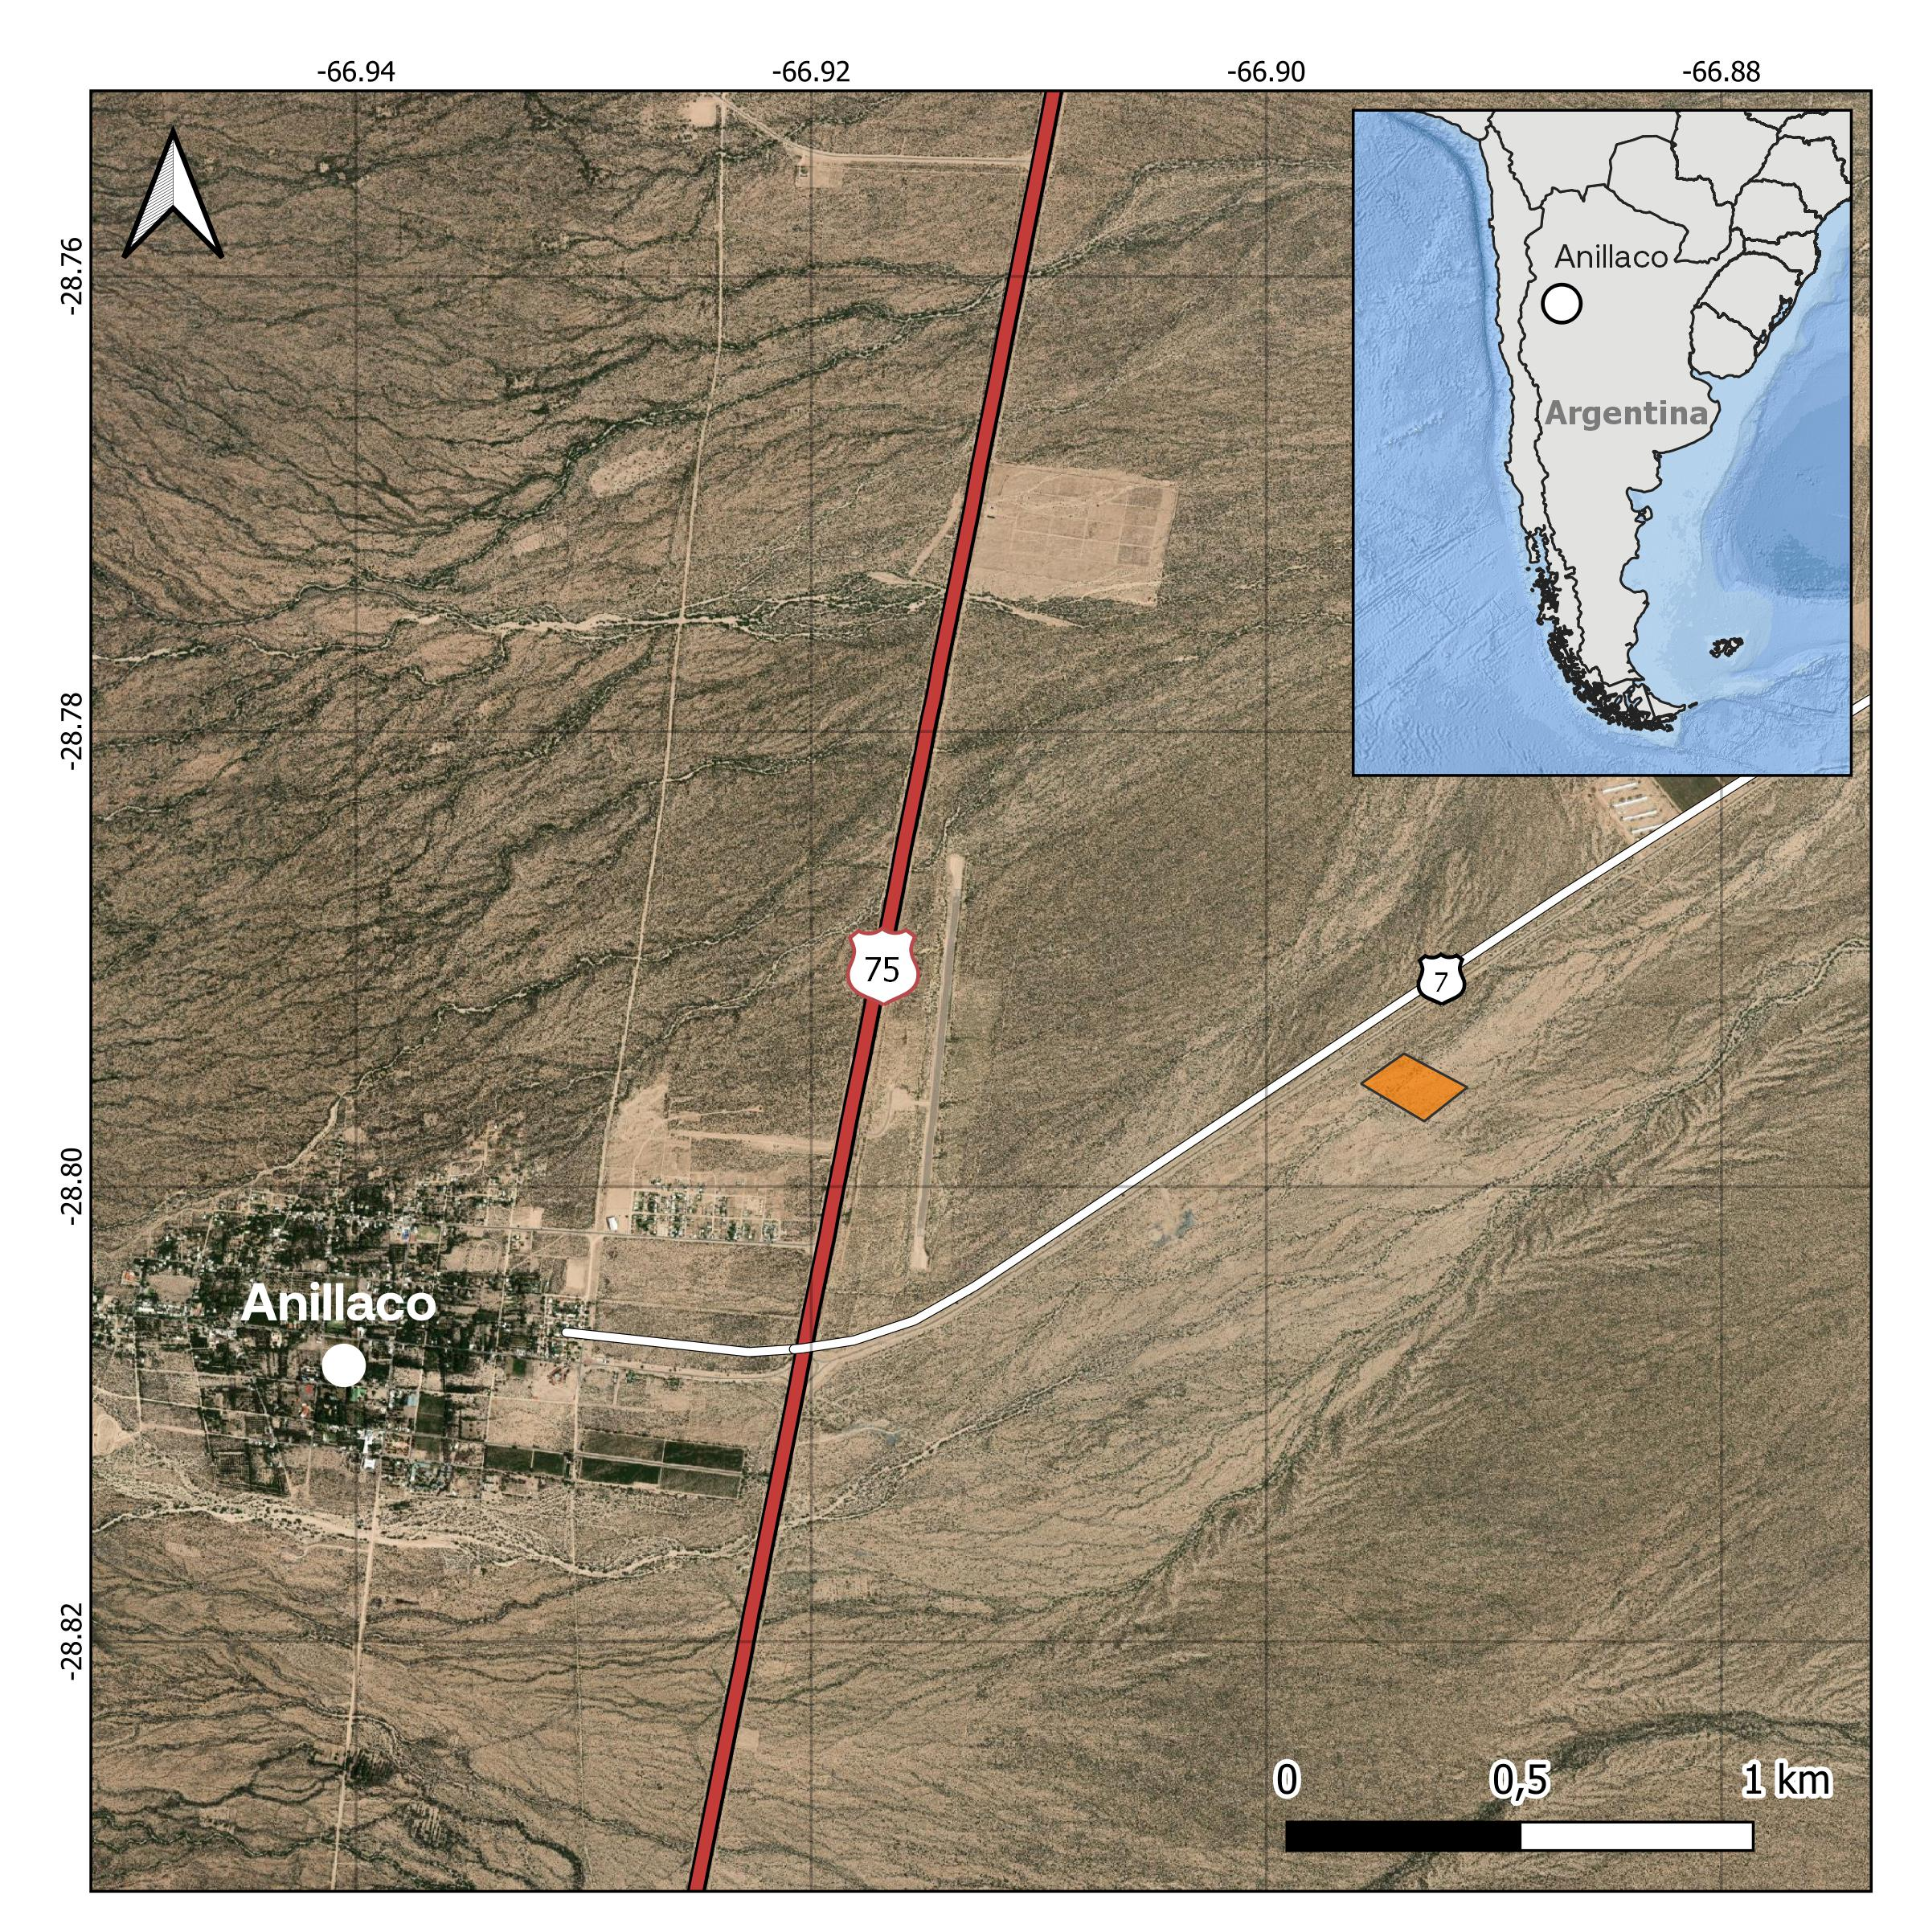
\includegraphics[width=1\linewidth]{../04_figures/map/tuco_map} 

  }

  \caption{Study site location (orange icon) at the Monte Desert, approximately 5km away form the village of Anillaco, northwest of Argentina}\label{fig:methods-map}
  \end{figure}
  \hypertarget{animal-capture-and-handling}{%
  \subsection{Animal Capture and Handling}\label{animal-capture-and-handling}}

  A total of 47 tuco-tucos were captured between March 2019 and March 2020. Out of these, 30 were part of the present study. Trapping was conducted in four different campaigns to the study site. Three campaigns were done in 2019 during March-April, July and October. A fourth campaign was done in February 2020. A fifth campaign was planned to occur in May 2020 but had to be canceled due to the COVID outbreak. Tuco-tucos were captured using a custom-made PVC tubing trap (35cm length, 10cm diameter) with a spring-loaded aluminum door at one end and a cul-de-sac at the other. Before setting the traps the study site was scouted for active tuco-tuco's burrows. Active burrows could be identified by the presence of freshly excavated soil mounds at the burrow's entrance. Once found burrows were excavated to open the access to the underground tunnels and a trap was placed horizontally at the burrow's entrance following the tunnel's orientation. Traps were placed at all active burrows found at the study site, limited to a max of 20 traps available. Traps were set in the field during the morning and checked every 2 hours, when they were reset if they had been plugged with soil or if they had been activated without any tuco-tuco capture. Traps were checked for a last time at dusk and then taken out if no animal had been caught.

  After capture, adult tucos (\textgreater120g) were first lightly anesthetized in order to be carefully examined and receive a biologging collar. We used a clear plastic anesthesia chamber (318.5cm³) with a clip-on lid and a cotton ball inside. The cotton ball received approximately 0.5 mL of isoflurane (\textbf{\emph{REF}}) before transferring the animal from the trap to the chamber. While in the chamber animals were observed for breathing, blinking and loss of righting reflex. Once the tuco-tucos could not right themselves they were removed from the chamber. Anesthetized animals were weighted (CSseries, OHAUS, ± 1 g precision), sexed, assesed for reproductive status, marked with a subcutaneous identification PITTag (Passive Integrative Transponder. Allflex, Brasil) and fitted with a collar bearing biologgers (See Activity Sensors).

  Animals were released in the same burrow they were originally captured. They were left in the field for 5-18 days before being recaptured for collar recovery. The telemetry transmitter were used to maximize the animals relocation, thus avoiding the loss of the other devices. All animal captures, procedures and animal handling were authorized by the local authorities at \emph{Dirección General de Ambiente y Desarrollo Sustentable -- Secretaría de Ambiente del Ministerio de Producción y Desarollo Local} -- La Rioja, Argentina (\#00501-17). All procedures were also approved by the Ethics Committee at the \emph{Instituto de Biociências} (\#308-2018) and \emph{Faculdade de Medicina Veterinária} (\#2045300519) of the \emph{Universidade de São Paulo}.

  \hypertarget{activity-sensors}{%
  \subsection{Activity Sensors}\label{activity-sensors}}

  Accelerometers (Axy-4, TechnoSmart, Italy) and lightloggers (W65, Migrate Technology, UK) were used to record general motor activity and light exposure, respectively. These biologgers were attached to a collar made of a cable tie inserted through silicon tubing (\protect\hyperlink{ref-jannetti2019}{Jannetti et al. 2019}; \protect\hyperlink{ref-williams2014}{Williams et al. 2014}). A telemetry transmitter (SOM-2011. Wildlife Materials, USA) was also attached to the collar to assist in animal location during recapture and minimize sensor's loss. The complete collar setup (accelerometer, lightlogger and telemetry) weighted approximately a total of 6g. Collars without the lightlogger weighted 5.3g. All accelerometers recorded tri-axial acceleration at a 10Hz sampling frequency with a 4G sensitivity. Lightloggers were set to sample light every minute but only recorded the maximum sampled value each 5 minutes.
  \begin{figure}

  {\centering 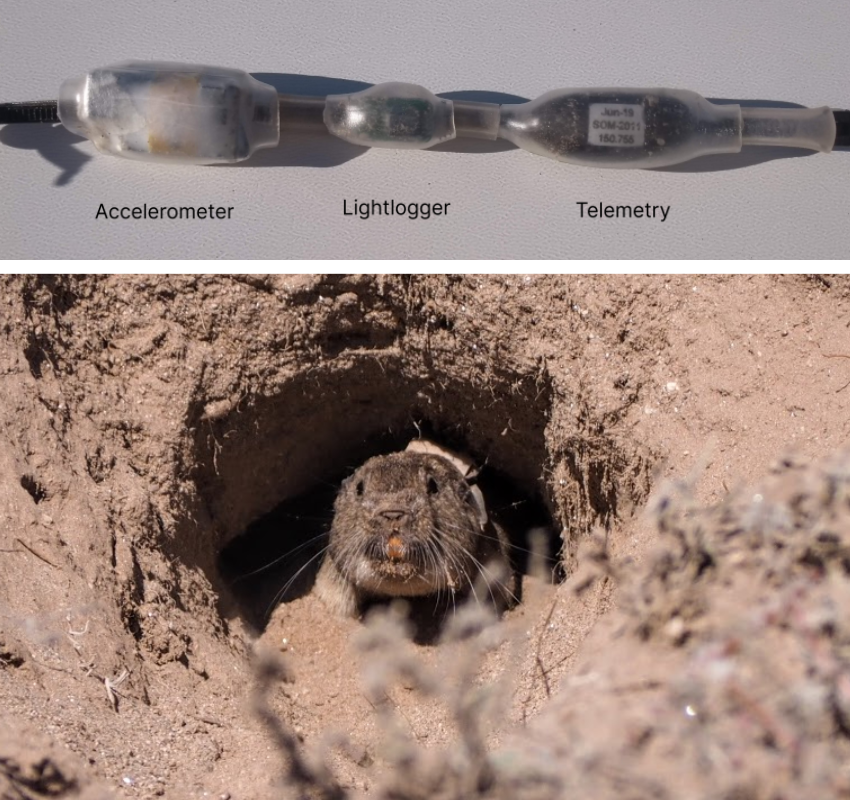
\includegraphics[width=1\linewidth]{../04_figures/collar/collar_tuco} 

  }

  \caption{Collar setup and field deployment. Upper photo shows the complete collar setup with both sensors and the telemetry transmitter. Bottom photo shows a tuco-tuco wearing a collar. In the bottom photo it is possible to see the acceleromer and the lightlogger attached to the collar.}\label{fig:methods-collar}
  \end{figure}
  \hypertarget{data-processing}{%
  \subsection{Data Processing}\label{data-processing}}

  Data were recorded on board of the sensors and later downloaded and converted to raw text files using the software provided by the logger manufacturers. Acceleration data was used to measure gross motor activity. Tri-axial acceleration data was first reduced to one dimension using the Vectorial Dynamic Body Acceleration (VeDBA, \protect\hyperlink{ref-qasem2012}{Qasem et al. 2012}). VeDBA is commonly used as a proxy for the animal's activity level and energy expenditure (\textbf{REFS}). VeDBA was calculated by: (i) Estimating the effect of the gravitational force over the accelerometer, also known as static acceleration. The static acceleration can be estimated by applying a moving average over the raw acceleration data. There is not a consensus over the the number of points to calculate the moving average with, which can be dependent on the study species and device's recording frequency. In this study we used a 4-second moving average after following the methodology proposed by (\protect\hyperlink{ref-shepard2008}{Shepard et al. 2008}, Fig. \ref{fig:appendix-smooth-window}). (ii) Calculating the acceleration correspondent to the animal's movement, also know as Dynamic Body Acceleration (DBA). The DBA was calculated by subtracting the static acceleration from the raw data. (iii) Lastly, we calculate the VeDBA by the vectorial sum of the DBA over the device's axes.

  \[ VeDBA = \sqrt{Xd^2 + Yd^2 + Zd^2} \]

  Once VeDBA was calculated, the 1Hz acceleration data was downsampled by taking the median over a 1 minute non-overlapping sliding window. All VeDBA datapoints were classified as occuring during the daytime or nighttime based on the daylength of recording dates. Daylength was calculated using the \emph{maptools} package in R (\protect\hyperlink{ref-bivand2020}{Bivand and Lewin-Koh 2020}), which uses the National Oceanic and Atmospheric Administration (NOAA) equations for estimating Twilight times. We used Civil Twilight times, defined as the times in which the center of the sun is 6° below the horizon, as thresholds to calculate daylength and classify datapoints as occuring during the day or nighttime. Daylength change along the year can be seen in the Appendix (\ref{fig:appendix-daylenght}).

  Light exposure data was used to further classify VeDBA data points as above or below ground. The threshold for considering a data point as being aboveground was 2 lux, consistent with what has been done in \protect\hyperlink{ref-jannetti2019}{Jannetti et al.} (\protect\hyperlink{ref-jannetti2019}{2019}).

  Accelerometer and lightlogger data were merged accordingly to the date and times of recordings using purposely written R scripts (\protect\hyperlink{ref-rcoreteam2020}{R Core Team 2020}). Time of recordings between both devices were not synchronized to the minute. Consequently, we had to round lightlogger recording times to the nearest 5 minutes in order to merge both data streams.

  In order exclude any effects that capture and recapture can have in the first days of recordings we removed the first and last days of each dataset. In cases where the recapture took longer than one day we also excluded the days that traps were set up in the animal's burrow. Exclusion of recapturing days corresponds to the last 5 days of two animals in February (FEV05 and JUL16); and the last 2 days of one animal in July (JUL23).

  \hypertarget{hidden-markov-models}{%
  \subsection{Hidden Markov Models}\label{hidden-markov-models}}

  In order to further analyze and classify the 1-minute VeDBA data we used Hidden Markov Models (HMMs). HMMs are a type of time series model, therefore, they take into account the temporal dependency of the observations (\protect\hyperlink{ref-leosbarajas2017}{Leos-Barajas et al. 2017}). Consequently HMMs are well suited to model accelerometer data given their natural temporal dependency (\protect\hyperlink{ref-leosbarajas2017}{Leos-Barajas et al. 2017}; \protect\hyperlink{ref-patterson2019}{A. Patterson et al. 2019}). HMMs are composed of two time series: the observable \emph{state-dependent process} (\(X_t\)), VeDBA in our case, and an underlying, or hidden, \emph{state process} (\(S_t\)). The \emph{state process} is what drives the observations and what we are interested in estimating, which roughly corresponds to behavioral states (Fig. \ref{fig:hmm-formulation}). We determined \emph{a priori} a possible number of three different states. This decision was made based on our research question, in the VeDBA distributions (Fig. \ref{fig:appendix-eda}) and in the biological interpretability of the states.

  The \emph{state process} follows the Markov Property and take temporal dependency into account (\protect\hyperlink{ref-zucchini2016}{Zucchini, Iain MacDonald, and Roland Langrock 2016}). The Markov property denotes that a state \(S_t\) depends only on the previous state \(S_{t-1}\) (\protect\hyperlink{ref-zucchini2016}{Zucchini, Iain MacDonald, and Roland Langrock 2016}). In the case of accelerometer and animal movement studies the states are representations of the animals' behavior and can take on finite number (\(N\)) of possible values. The number of states can be chosen \emph{a priori} or based on model selection (\protect\hyperlink{ref-pohle2017}{Pohle et al. 2017}). The changes in probabilities between states are also part of the of HMM formulation, summarized by a Transition Probability Matrix that gives the probability of transitioning from the current state to a possible future state.

  In the basic HMM formulation the observable \emph{state-dependent process} comes from a mixture of \(N\) distributions, one for each state. These distributions come from a common family (e.g.~Normal, Weibull or Gamma) and each one have their own set of parameter values. The active distribution is determined by the state the system is in at a given time \(t\). The observations therefore are a realization from one of these distributions. The distribution parameters, state transition probabilities and other model parameters can be estimated by numerical maximization of the Likelihood (\protect\hyperlink{ref-zucchini2016}{Zucchini, Iain MacDonald, and Roland Langrock 2016}). With the model parameters in hand, the most probable state sequence can be found by the Viterbi algorithm (\protect\hyperlink{ref-mcclintock2020}{Brett T. McClintock et al. 2020}; \protect\hyperlink{ref-zucchini2016}{Zucchini, Iain MacDonald, and Roland Langrock 2016}).
  \begin{figure}

  {\centering 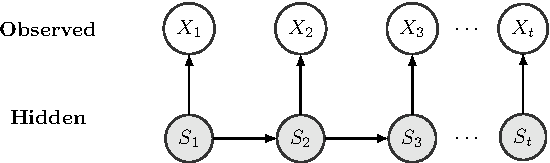
\includegraphics{tese_jefferson_files/figure-latex/hmm-formulation-1} 

  }

  \caption{Basic dependence structure for a Hidden Markov Model}\label{fig:hmm-formulation}
  \end{figure}
  \hypertarget{model-formulation-and-state-classification}{%
  \subsection{Model Formulation and State Classification}\label{model-formulation-and-state-classification}}

  In our models we have chosen VeDBA as our activity metric. To model the VeDBA we determined \emph{a priori} that the hidden \emph{state-process} could assume three different states (\(N=3\)). It is important to note that states do not correspond directly to specific behaviors (e.g.~feeding, foraging or digging) but can be assumed to roughly correspond to behavioral states (e.g.~activity levels) that can encompass a range of different behaviors (\protect\hyperlink{ref-leosbarajas2017}{Leos-Barajas et al. 2017}; \protect\hyperlink{ref-papastamatiou2018}{Papastamatiou et al. 2018}). We labelled the states as roughly corresponding to ``Rest,''``Medium Intensity Activity'' and ``High Intensity Activity.''

  HMMs can be fitted individually (e.g. \protect\hyperlink{ref-vandekerk2015}{van de Kerk et al. 2015}) or to a pool of animals (\protect\hyperlink{ref-langrock2012}{Langrock et al. 2012}). The models can also include covariate effects that modify either the \emph{state-dependent} distribution parameters or the transition probabilities (\protect\hyperlink{ref-patterson2009}{T. A. Patterson et al. 2009}; \protect\hyperlink{ref-langrock2012}{Langrock et al. 2012}). We fitted a 3-state HMM to the 1-minute VeDBA data using a `complete pooling' approach. This means that the \emph{state-dependent} distribution parameters are common to all animals. Therefore we assume that individuals are independent and behaviors are the same to all individuals and across the year. However, given that the season/month of the year seems to be an important feature influencing the VeDBA distribution (Fig. \ref{fig:appendix-eda}) we included season as a covariate in the \emph{state process}. Hence we let the probability of changing from one state to another vary in relation to the season/month of the year. We also fitted an empty model, with no covariate effects, and used Akaike's Information Criteria (AIC) to select the model with best fit to the data (\protect\hyperlink{ref-burnham2002}{Burnham, Anderson, and Burnham 2002}).

  Models were fitted using the momentuHMM package in R (\protect\hyperlink{ref-mcclintock2021}{Brett T. McClintock and Michelot 2021}). We used the gamma distribution, parametrized with mean and standard deviation, to model VeDBA. The gamma distribution is a flexible distribution, usually used in movement studies (\textbf{REFS}), that accommodates positive right-skewed data. Appropriate starting values for likelihood maximization of model's parameters were found by following procedures suggested by \protect\hyperlink{ref-michelot2019}{Michelot and Langrock} (\protect\hyperlink{ref-michelot2019}{2019}). Season was included as a categorical variable, its influence over the transition probabilities was summarized using stationary probabilities plots (\protect\hyperlink{ref-leosbarajas2017}{Leos-Barajas et al. 2017}). The most probable state sequence was decoded using the Viterbi algorithm (\protect\hyperlink{ref-zucchini2016}{Zucchini, Iain MacDonald, and Roland Langrock 2016}). The decoded sequence was then used to conducted other \emph{post-hoc} analysis of diurnality and rhythmicity. We checked model assumptions and goodness of fit by visual inspection of the pseudo-residuals (\protect\hyperlink{ref-zucchini2016}{Zucchini, Iain MacDonald, and Roland Langrock 2016}).
  \begin{itemize}
  \tightlist
  \item
    michelot 2 017 - Estimation and simulation of foraging trips in land-based marine predators. Ecology 98, 1932--1944. \href{https://doi.org/10.1002/ecy.1880}{doi.org/10.1002/ecy.1880}
  \end{itemize}
  \hypertarget{diurnality-index}{%
  \subsection{Diurnality Index}\label{diurnality-index}}

  Diurnality was calculated

  \hypertarget{rhythmicity}{%
  \subsection{Rhythmicity}\label{rhythmicity}}

  (\ldots)

  \hypertarget{statistical-analysis}{%
  \subsection{Statistical Analysis}\label{statistical-analysis}}

  First we tested for differences in mean daily VeDBA between season with an ANOVA followed by a post-hoc Tukey-Kramer's test. Next, with the state-labelled VeDBA data in hand, we tested for seasonal differences between the proportion of time spent in each state with an ANOVA and post-hoc Tukey-Kramer's test.

  \hypertarget{results}{%
  \section{Results}\label{results}}
  \begin{itemize}
  \tightlist
  \item
    Ao adicionar numero de animais tbm comentar da dificuldade em recapturar e em alguns casos capturar machos! Legal para futuras referencias. (Talvez nos resultados?)
  \end{itemize}
  During 2019-2020, we captured 30 tucos, 20 females and 10 males. Each tuco received a biologging collar, mostly containing an accelerometer and a lightlogger. We were able to recapture 24 tucos and recover 21 collars (Table \ref{tab:table-captures}). One collar was lost because one tuco got predated and the collar was found malfunctioning. The other two lost collar fell or were taken out of the tuco's neck between the time of capture and recapture. All 21 animals that were recapture received a collar containing an accelerometer. However, only 13 also received a lightlogger (Table \ref{tab:table-captures}). In total we have 13 complete datasets, with acceleration and light exposure data, and 8 datasets with only acceleration data.
  \begin{table}[h]
  \centering
  \caption{Number of captured animals and sensors deployed in the field. There was a higher number of females captured independent of the season. Recapture rates in February 2021 are lower because field work had to be interrupted due to the covid outbreak. Not all recaptured tucos still had their collars. Some collar were taken out by the animals between the time of captured and recaptured. One tuco was predated and the collar was found 1km away from the initial capture burrow malfunctioning.}
  \label{tab:table-captures}
  \resizebox{\textwidth}{!}{%
  \begin{tabular}{llllllll} 
  \toprule
           & \multicolumn{2}{c}{Captured}                            & \multicolumn{2}{c}{Recaptured}                          &                                       &                                    &                                   \\ 
  \cmidrule{2-5}
      & \multicolumn{1}{c}{Males} & \multicolumn{1}{c}{Females} & \multicolumn{1}{c}{Males} & \multicolumn{1}{c}{Females} & \multicolumn{1}{c}{Recovered Collars} & \multicolumn{1}{c}{Accelerometers} & \multicolumn{1}{c}{Lightloggers}  \\ 
  \midrule
  February & 3                         & 7                           & 2                         & 5                           & 5                                     & 5                                  & 5                                 \\
  July     & 4                         & 5                           & 4                         & 5                           & 8                                     & 8                                  & 6                                 \\
  March    & 0                         & 2                           & 0                         & 2                           & 2                                     & 2                                  & 0                                 \\
  October  & 3                         & 6                           & 1                         & 5                           & 6                                     & 6                                  & 2                                 \\
  \bottomrule
  \end{tabular}
  }
  \end{table}
  \hypertarget{daily-activity-levels}{%
  \subsection{Daily Activity Levels}\label{daily-activity-levels}}

  Tuco's activity levels are significantly lower during July in comparison to other months. Accelerometer data was used to calculated the Vectorial Dynamic Body Acceleration (VeDBA) that we use as a proxy for animal activity. Tuco's daily activity levels (24h average), measured by VeDBA, are significantly different across the year (ANOVA; F = 7.182, p \textless{} 0.01; Fig. \ref{fig:vedba-boxplot}). Post hoc comparisons using Tukey-Kramer's Test shows significant group differences between July-October and July-February (p \textless{} 0.05). In both pairwise comparisons July Daily VeDBA levels are lower, showing a difference in means of 0.029g and 0.019g in comparison to October and February, respectively. In sum, daily VeDBA activity levels are lower in July in comparison to October and February (Fig \ref{fig:vedba-boxplot}).
  \begin{itemize}
  \tightlist
  \item
    Tirar?:
  \end{itemize}
  The daytime VeDBA (Light Phase Average) is also significantly different between Months (ANOVA; F = 7.282, p \textless{} 0.001). Post hoc comparisons using Tukey-Kramer's Test shows a difference in mean of 0.035 between October-July (p \textless{} 0.05). However, daytime activity levels are only significantly different between July and October.
  \begin{figure}

  {\centering 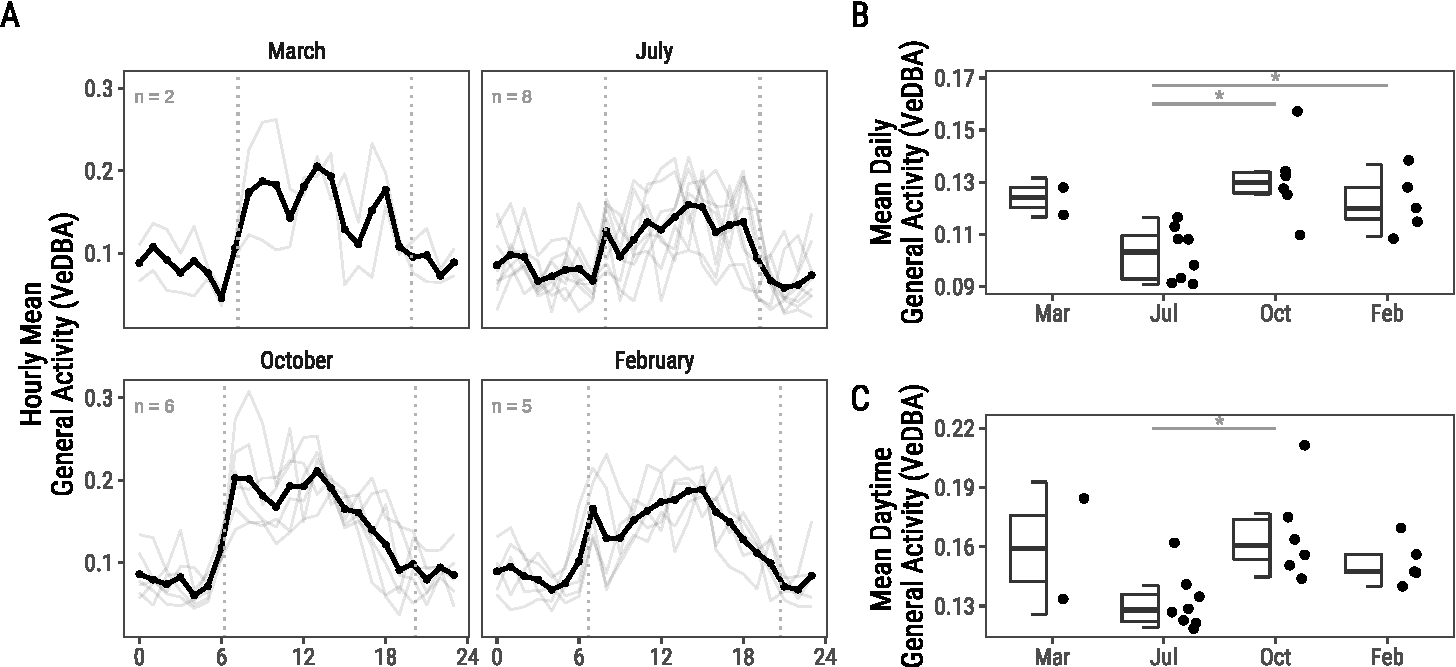
\includegraphics[width=1\linewidth]{tese_jefferson_files/figure-latex/vedba-boxplot-1} 

  }

  \caption{Tuco-tuco's Daily VeDBA levels. (A) VeDBA was binned by hour (0-23). Background lines show data for individual animals. Thick lines show mean hourly VeDBA. (B) Points show daily (24h) VeDBA mean for each animal. In July Tuco-tuco's exhibited lower Daily VeDBA than October and February. Dashed lines in Panel A shows time of civil dawn and dusk.}\label{fig:vedba-boxplot}
  \end{figure}
  \hypertarget{state-classification}{%
  \subsection{State Classification}\label{state-classification}}

  We modeled and classified VeDBA into three distinct behavioral states using Hidden Markov Models (HMM). We fitted two different models, one empty model, with no covariates, and a second one with \emph{`season'} as a covariate in the transition probability matrix. The second model was selected based on informational criterion (\(\Delta\)AIC \textgreater{} 2; REF Tabela AIC nos supps).

  The estimated state-dependent distributions are shown in Figure \ref{fig:hmm-plot}. We interpreted and labelled these states as `rest,' `medium intensity activity,' and `high intensity activity' corresponding to low, intermediate and high VeDBA values respectively. The marginal distribution (Fig. \ref{fig:hmm-plot}; dashed line) has a good correspondence to the empirical VeDBA distribution. A visual analysis of the Pseudo-residuals (Fig. \ref{fig:appendix-residuals}) show that the residuals deviates from the expected normal distribution, especially in the lower end values, and that there is still significant residual autocorrelation. Nevertheless, the overall fitting seems to be reasonable. The estimated state-dependent parameters are shown in the Appendix (Table \ref{tab:appendix-parameters}).
  \begin{figure}

  {\centering 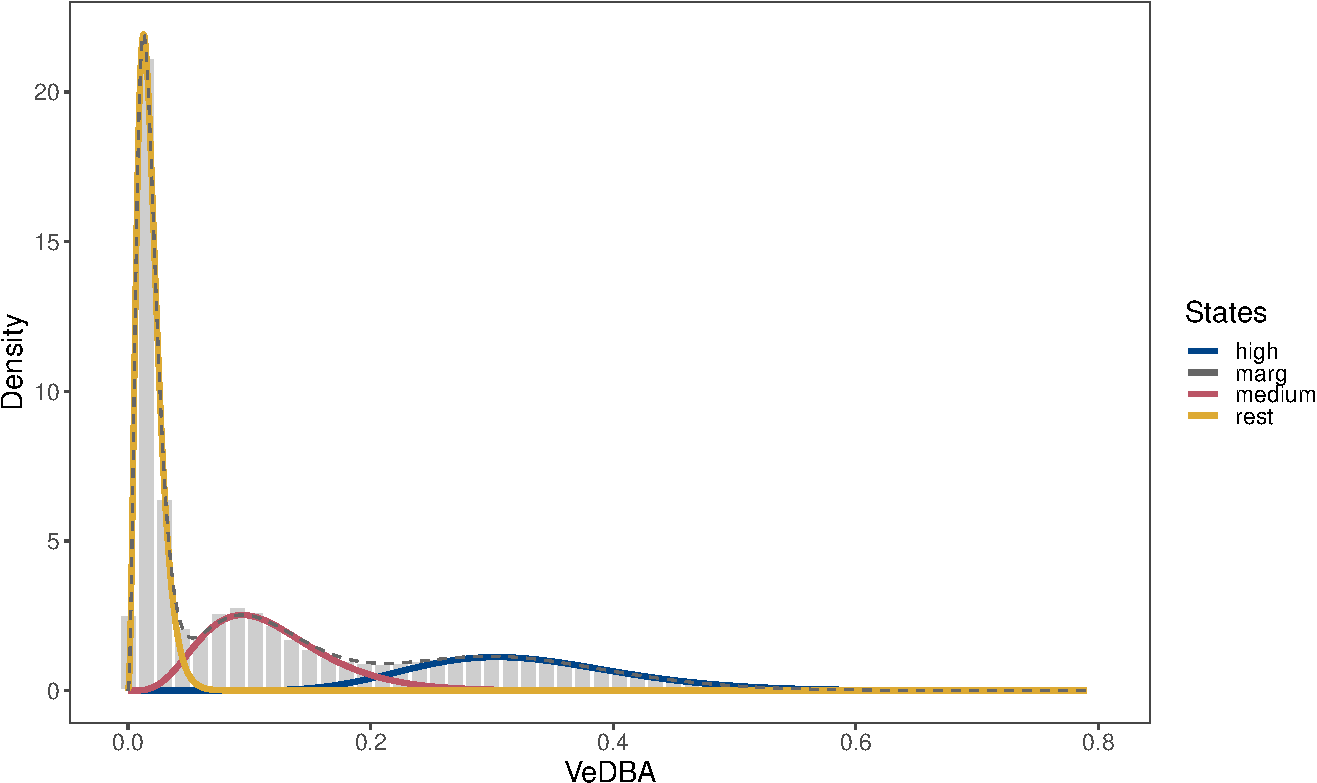
\includegraphics[width=1\linewidth]{tese_jefferson_files/figure-latex/hmm-plot-1} 

  }

  \caption{State-dependent distributions of the selected Hidden Markov model fitted to the VeDBA acceleration metric. Histogram, in grey, shows the Vectorial Dynamic Body Acceleration (VeDBA) from the data of 21 Anillaco's tuco-tuco. State-dependent gamma distributions are shown above the histograms. These distributions are weighted accordingly to the proportion of observations assigned to each state.}\label{fig:hmm-plot}
  \end{figure}
  We labelled VeDBA data using the Viterbi algorithm. With the state-labeled data we were able to disassociated and visualize the daily patterns of each different state. Time series plots and actograms, a classic form of visualization in chronobiology, shows how the different states are related to the calculated VeDBA. We can also begin to qualitatively evaluate diel rhythms in VeDBA and in the state-labelled data. Figure \ref{fig:actograms-results} shows one representative animal's actograms and time series plot. Visually, the daily rhythm is more defined in High Activity in comparison to Medium Activity. However, despite being more concentrated during the daylight hours, High Activity episodes also occurs sporadically during the night. Medium Activity, in turn, seems to be more disperse throughout the day with no clear daily rhythm. Individual Actograms for VeDBA and state-labelled data are presented in the Appendix (Figure \ref{fig:vedba-actograms}).
  \begin{figure}

  {\centering 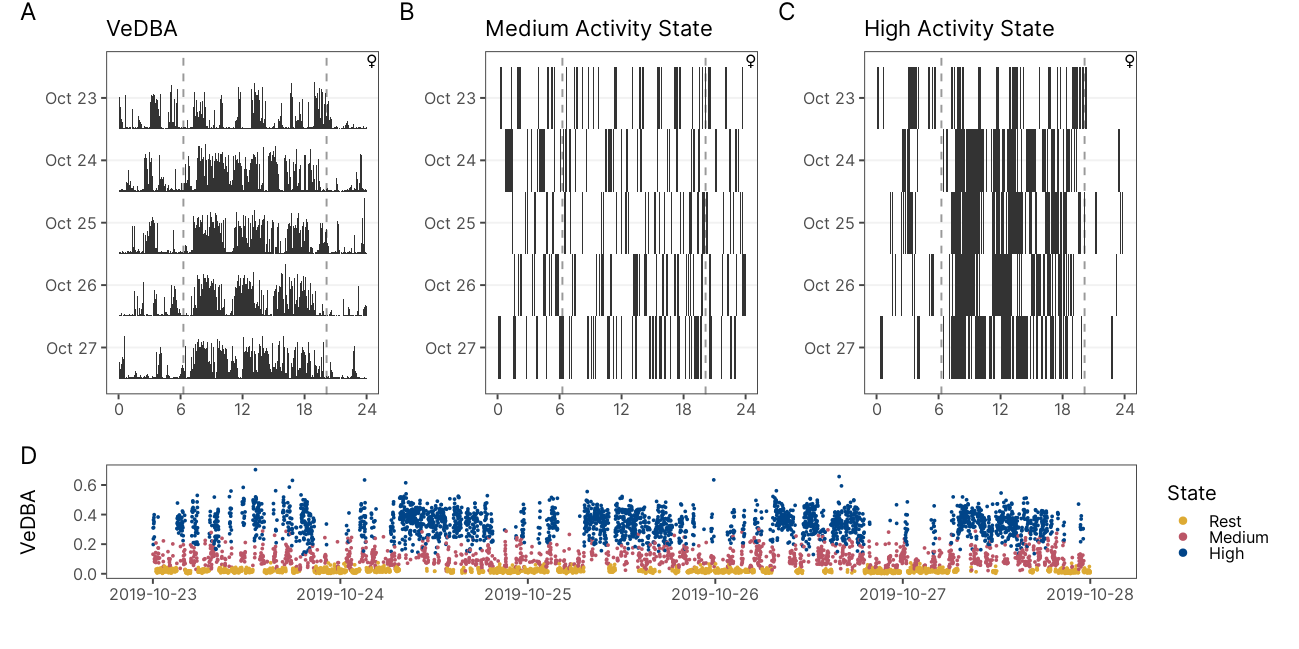
\includegraphics[width=1\linewidth]{../04_figures/actograms/actograms_results} 

  }

  \caption{Actograms and Time Series Plot of VeDBA and state-labelled data of a representative animal (ID:OCT09). The actograms shows daily patterns of VeDBA (A) and of Medium and High State occurrences (B and C). Medium Activity State shows no clear pattern of a daily rhythm. High Activity is disperse throughout the day with a higher concentration during daylight hours. The time series (D) shows state-labelled VeDBA data. Dashed lines shows time of dawn and dusk.}\label{fig:actograms-results}
  \end{figure}
  \clearpage

  \hypertarget{daily-time-activity-budgets}{%
  \subsection{Daily Time-Activity Budgets}\label{daily-time-activity-budgets}}

  Using the state-labelled data we calculated that on average tucos spent between 45-50\% of the 24 hours resting, depending on the month. The remaining time is spent in an active state, either Medium or High Activity State (Table \ref{tab:table-time-state}). ANOVA test shows no statistical difference between the percentage of time spent resting between groups (ANOVA; F = 1.93, p = 0.163).

  Tuco-tucos spent a variable percentage of their daily active time in one of the two active state, High or Medium Activity, across seasons. Daily time spent in High Activity was lower in July (15.8\%) and higher in October (29.4\%; \ref{tab:table-time-state}). In contrast, daily time spent in a Medium Activity State was higher in July (34.1\%) and lower in October (24.8\%). There is a significant difference in the percentage of time spent in Medium (Fig. \ref{fig:plot-time-state}; ANOVA: F = 4.457, p = 0.0175) and High Activity State (Fig. \ref{fig:plot-time-state}; ANOVA: F = 13.62, p = \textless{} 0.001). Tukey's post hoc test shows that the mean percentage of time spent in the Medium Activity State is 9\% lower in October than in July (p = 0.01). For the High Activity State, pairwise Tukey's test shows a significant difference between October-July (p \textless{} 0.001) and February-July (p \textless{} 0.01). In comparison to July the mean daily percentage of time spent in a High Activity State is 13\% higher in October and 8\% higher in February (Fig. \ref{fig:plot-time-state}).
  \begin{table}[!h]

  \caption{\label{tab:table-time-state}Average percentage of time spent in each state.}
  \centering
  \begin{tabular}[t]{cccccc}
  \toprule
  season & n & Rest & Medium & High & Active\\
  \midrule
  March & 2 & 45.01 & 32.06 & 22.94 & 55.00\\
  July & 8 & 50.09 & 34.13 & 15.78 & 49.91\\
  October & 6 & 45.78 & 24.78 & 29.44 & 54.22\\
  February & 5 & 45.14 & 30.18 & 24.68 & 54.86\\
  \bottomrule
  \end{tabular}
  \end{table}
  \begin{figure}

  {\centering 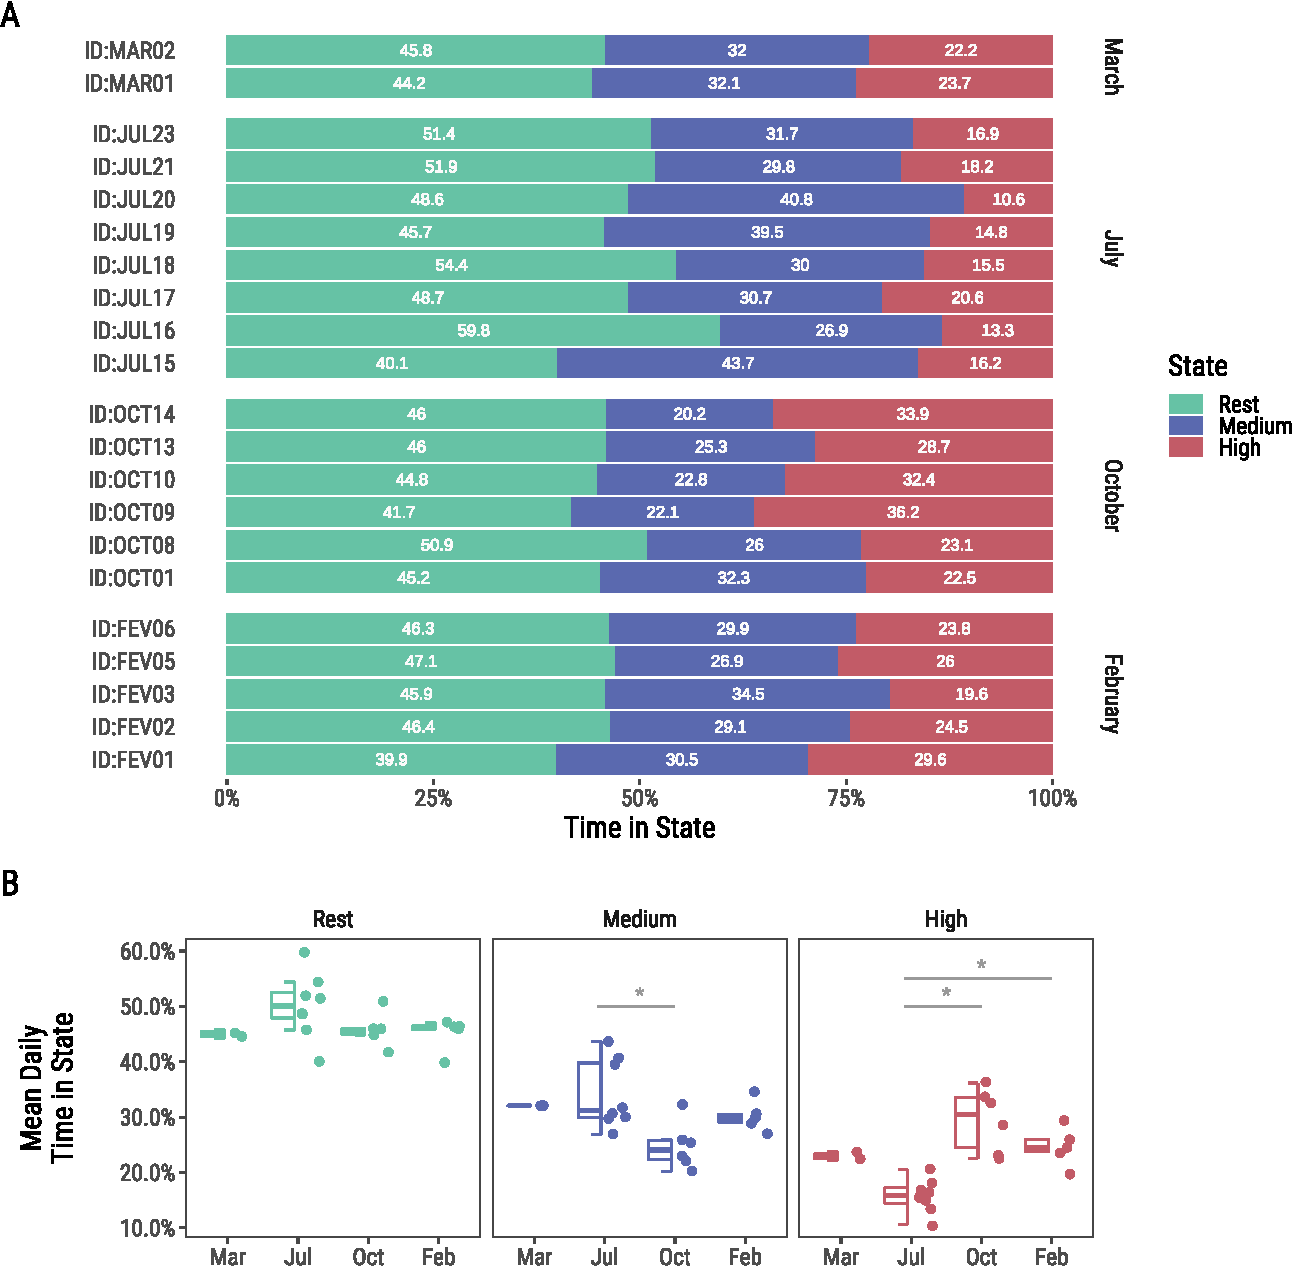
\includegraphics[width=1\linewidth]{tese_jefferson_files/figure-latex/plot-time-state-1} 

  }

  \caption{Daily time-activty budgets for the behavioral states. (A) Percentage of time spent in each behavioral state per animal. (B) Distribution of the mean percentage of time spent in each behavioral state calculated by animal. The mean pecentage of time spent in the High Activity State is lower in July in comparison to October and February. The mean percentage of time spent in the Medium Activity State, however, is higher in July in comparison with October.}\label{fig:plot-time-state}
  \end{figure}
  \newpage

  \hypertarget{daily-activity-patterns}{%
  \subsection{Daily Activity Patterns}\label{daily-activity-patterns}}

  Daily activity rhythms for each behavioral state is shown in Figures REF. These plots show that, qualitatively, when considered separately the timing of occurrence of High Activity and Light Exposure episodes follow a diurnal pattern. Medium Activity, however, is spread out along the 24h and do not follow a daily (24h) rhythm. It is important to note that the timing of peak occurrence of High Activity behavior does not appear to change dramatically along the year. In all four Months the peak of High Activity seems to be around 14:00. In turn, Light Exposure patterns changes along the year. In July, the peak of episodes of light exposure is more concentrated in the middle of the day. In other seasons the peak of Light Exposure episodes appears to be multimodal, with a higher peak in the first hours of daylight and a much smaller peak at the end of daylight.
  \begin{itemize}
  \tightlist
  \item
    calculate peak
  \item
    adicionar linha do meio dia solar
  \end{itemize}
  \begin{figure}

  {\centering 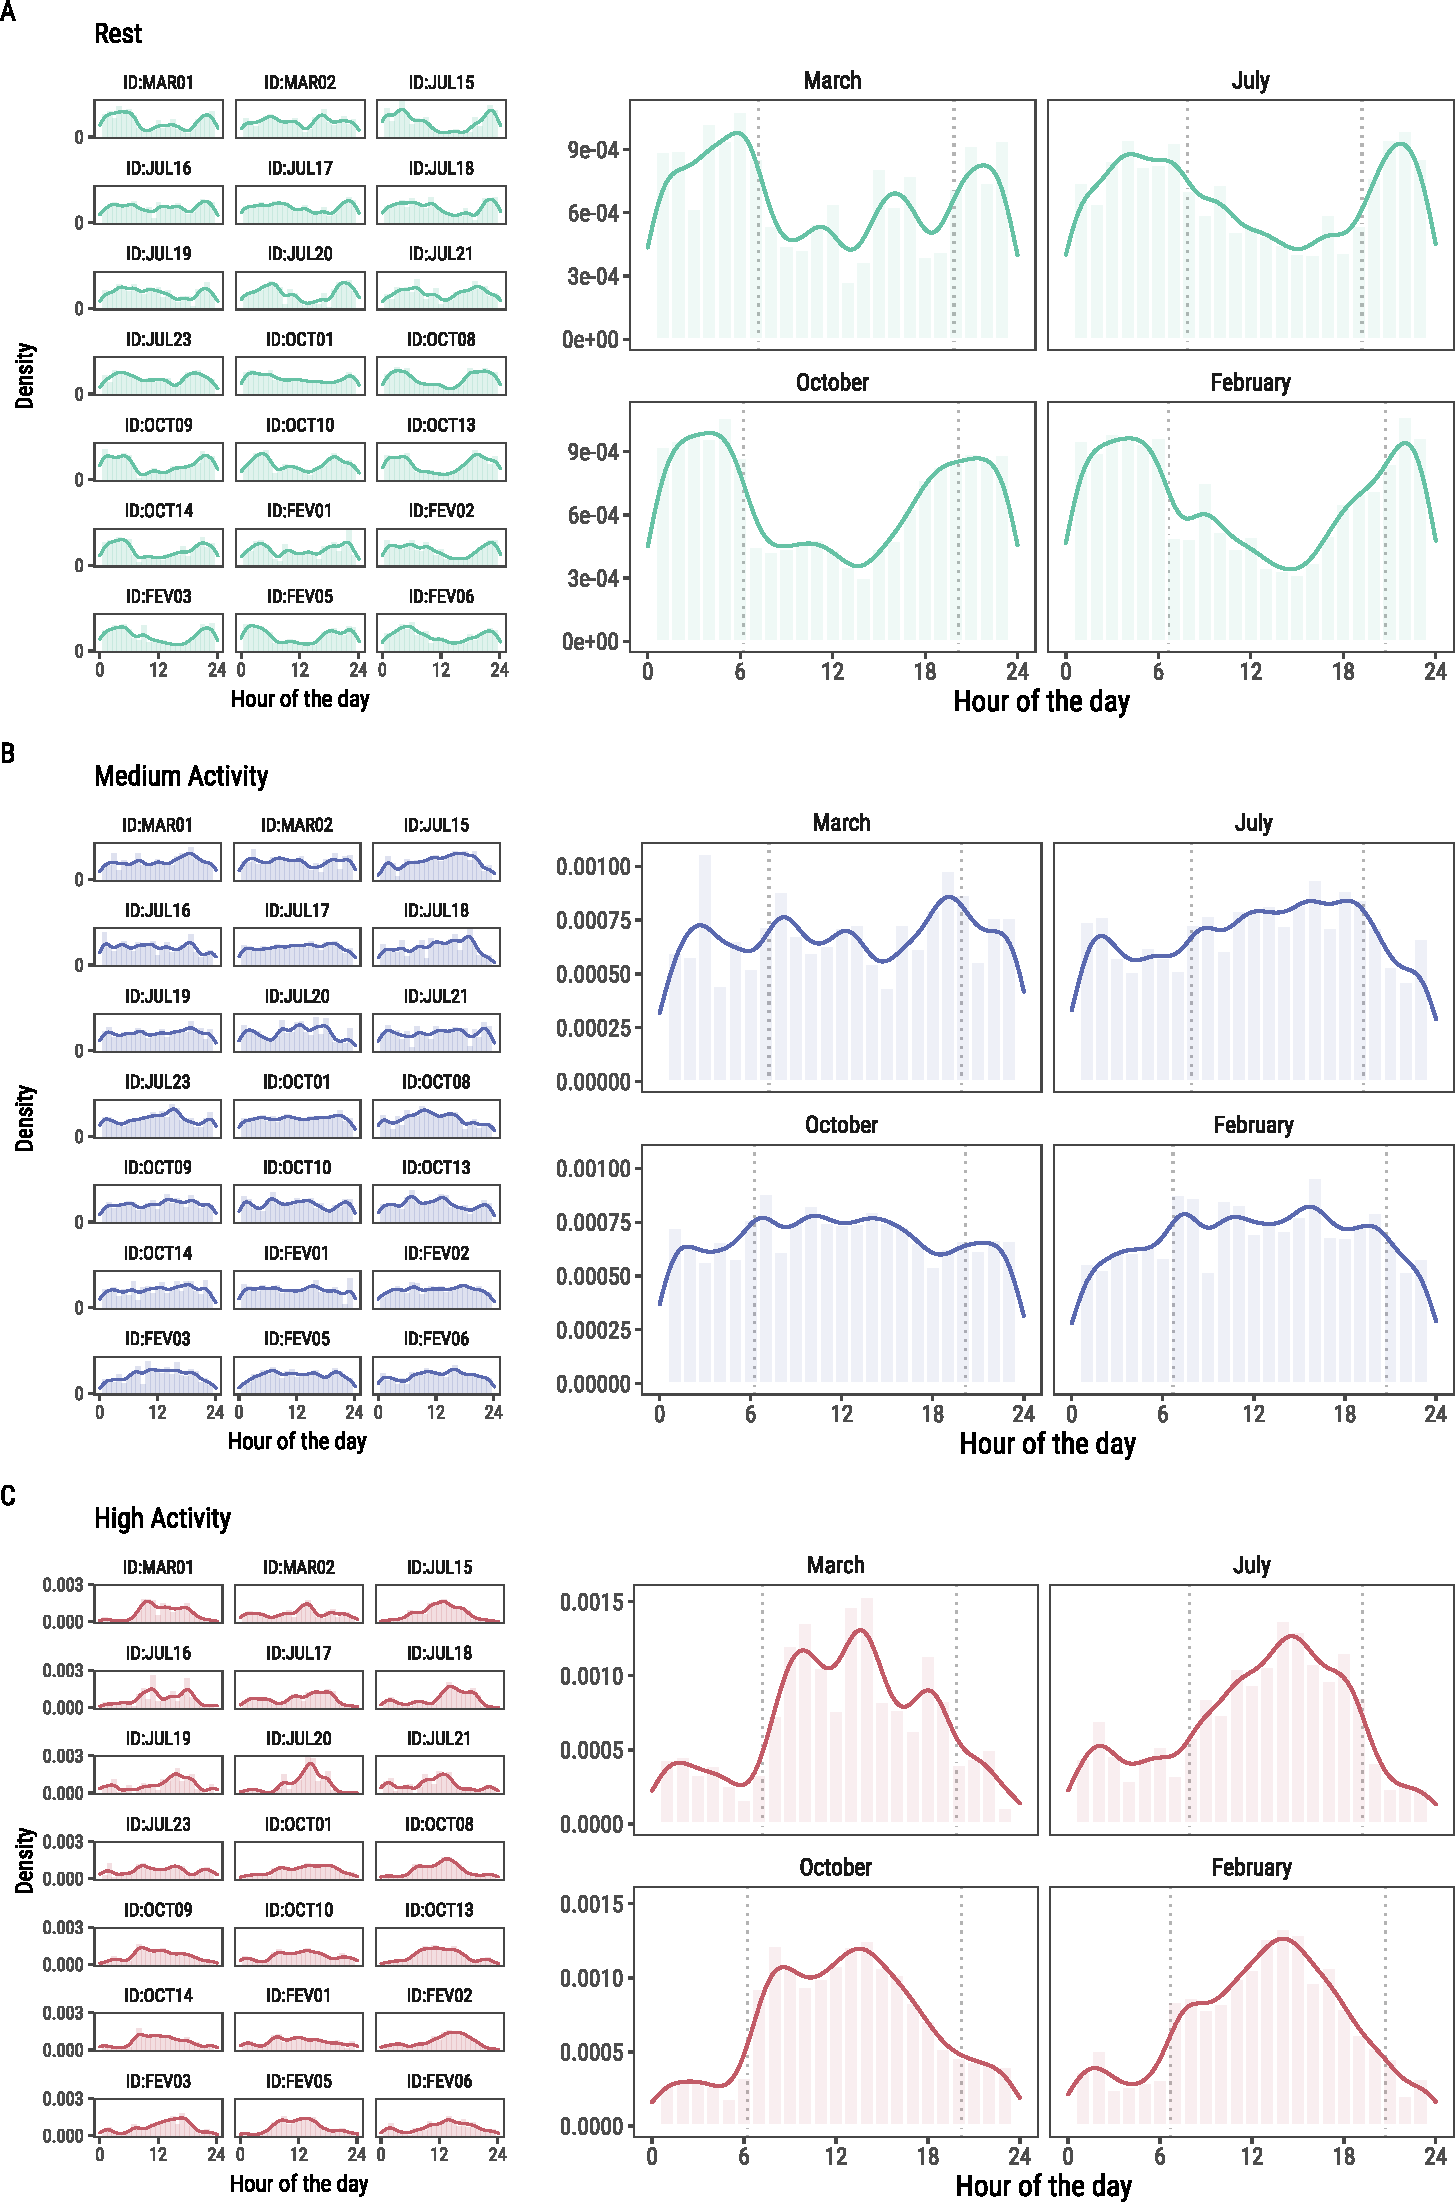
\includegraphics[width=0.85\linewidth]{tese_jefferson_files/figure-latex/plot-patterns-1} 

  }

  \caption{Density estimate of daily activity patterns of tuco-tucos' behavioral states. Solid lines indicate the Gaussian kernel density estimates. Light-colored bars show observed distribution of each beavioral state occurance. Rug lines above the x-axis shows individual occurances. Dotted vertical lines show time of civil twilights. High Activity State shows a diurnal pattern independent of the time of the year. Medium Activty State shows no daily pattern. Light Exposure shows a diurnal rhythm that changes according to the season. }\label{fig:plot-patterns}
  \end{figure}
  \newpage

  \hypertarget{diurnality}{%
  \subsection{Diurnality}\label{diurnality}}

  Only the High Activity State behavior is predominately diurnal. The average diurnality for the High Activity State is higher than 70\% for all seasons (Table \ref{tab:table-mean-time-in-state}). Medium Activity is evenly spread out along the 24h with a diurnality that ranges from 50\% in March to 56\% in July and February (Table \ref{tab:table-mean-time-in-state}). The Rest State is predominantly nocturnal with Diurnality lower than 38\% for all season. An ANOVA test show no difference in the mean diurnality between Months for each state (Figure \ref{fig:diurnality-plot}).
  \begin{figure}[H]

  {\centering 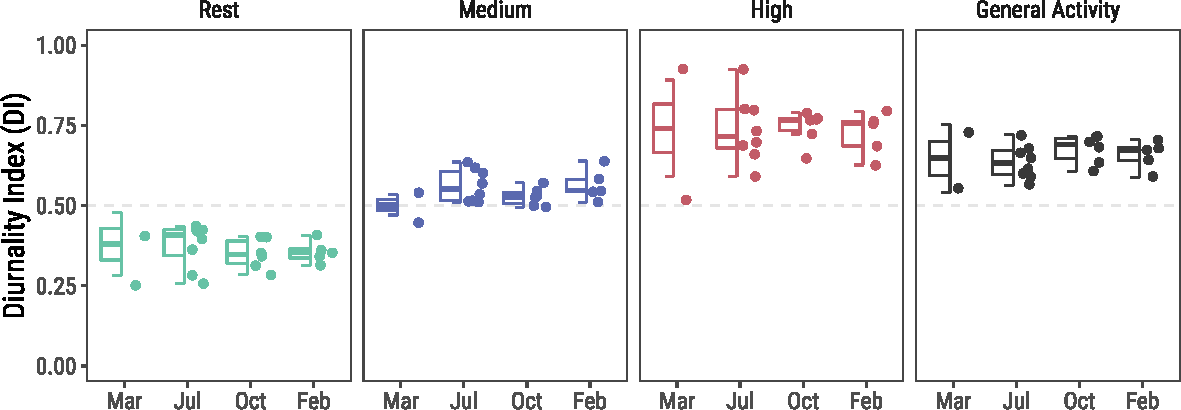
\includegraphics[width=0.95\linewidth]{tese_jefferson_files/figure-latex/diurnality-plot-1} 

  }

  \caption{Distriution of each state's diurnality. Only the High Activity State is predominatly diurnal. High Activity State had a average diurnality greater than 70\% for all season.}\label{fig:diurnality-plot}
  \end{figure}
  \begin{table}[!h]

  \caption{\label{tab:table-mean-time-in-state}Mean diurnality of each state.}
  \centering
  \begin{tabular}[t]{ccc}
  \toprule
  Season & State & Mean Diurnality\\
  \midrule
  March & rest & 0.38\\
  March & medium & 0.50\\
  March & high & 0.74\\
  July & rest & 0.38\\
  July & medium & 0.56\\
  \addlinespace
  July & high & 0.74\\
  October & rest & 0.35\\
  October & medium & 0.53\\
  October & high & 0.74\\
  February & rest & 0.35\\
  \addlinespace
  February & medium & 0.56\\
  February & high & 0.73\\
  \bottomrule
  \end{tabular}
  \end{table}
  \hypertarget{rhythmicity-1}{%
  \subsection{Rhythmicity}\label{rhythmicity-1}}

  (\ldots)

  \hypertarget{discussion}{%
  \section{Discussion}\label{discussion}}
  \begin{itemize}
  \tightlist
  \item
    Optamos pelo tipo de modelos mais simples com outras a analises a posteriori. Existem outros métodos interessantes Patterson 2009. Extensions to out model could include (\ldots)
  \item
    limitações dos dados de lightlogger: não sabemos se os picos podem se extender durante a noite tbm.
  \end{itemize}
  \appendix \# Apêndice \{-\}

  \hypertarget{anillacos-plant-community}{%
  \chapter{Anillaco's Plant Community}\label{anillacos-plant-community}}

  Following methods similar to (\protect\hyperlink{ref-aranda-rickert2014}{Aranda-Rickert, Diez, and Marazzi 2014}) a non-extensive survey of the plant community was done in May 2019. Three perpendicular 50m transects were defined near the study site (COORDINATES). A point-intercept method was used to record plant species present in the transects, species right below the sampling points were registered in the data. Sampling points were defined every 1m along the 50m transects. Plant species were identified in the field by a Botanist, except for a few members of the Poaceae family.

  The results for the plant survey is in line with what has been described in the literature for the region (\protect\hyperlink{ref-abraham2009}{Abraham et al. 2009}; \protect\hyperlink{ref-aranda-rickert2014}{Aranda-Rickert, Diez, and Marazzi 2014}; \protect\hyperlink{ref-fracchia2011}{Fracchia et al. 2011}). The results show a dominance of Zygolhyllaceae, Poaceae and Fabaceae families. The relative frequency of plant families and species recorded in the area are shown in the graphs below (Fig. \ref{fig:appendix-plants}).
  \begin{figure}

  {\centering 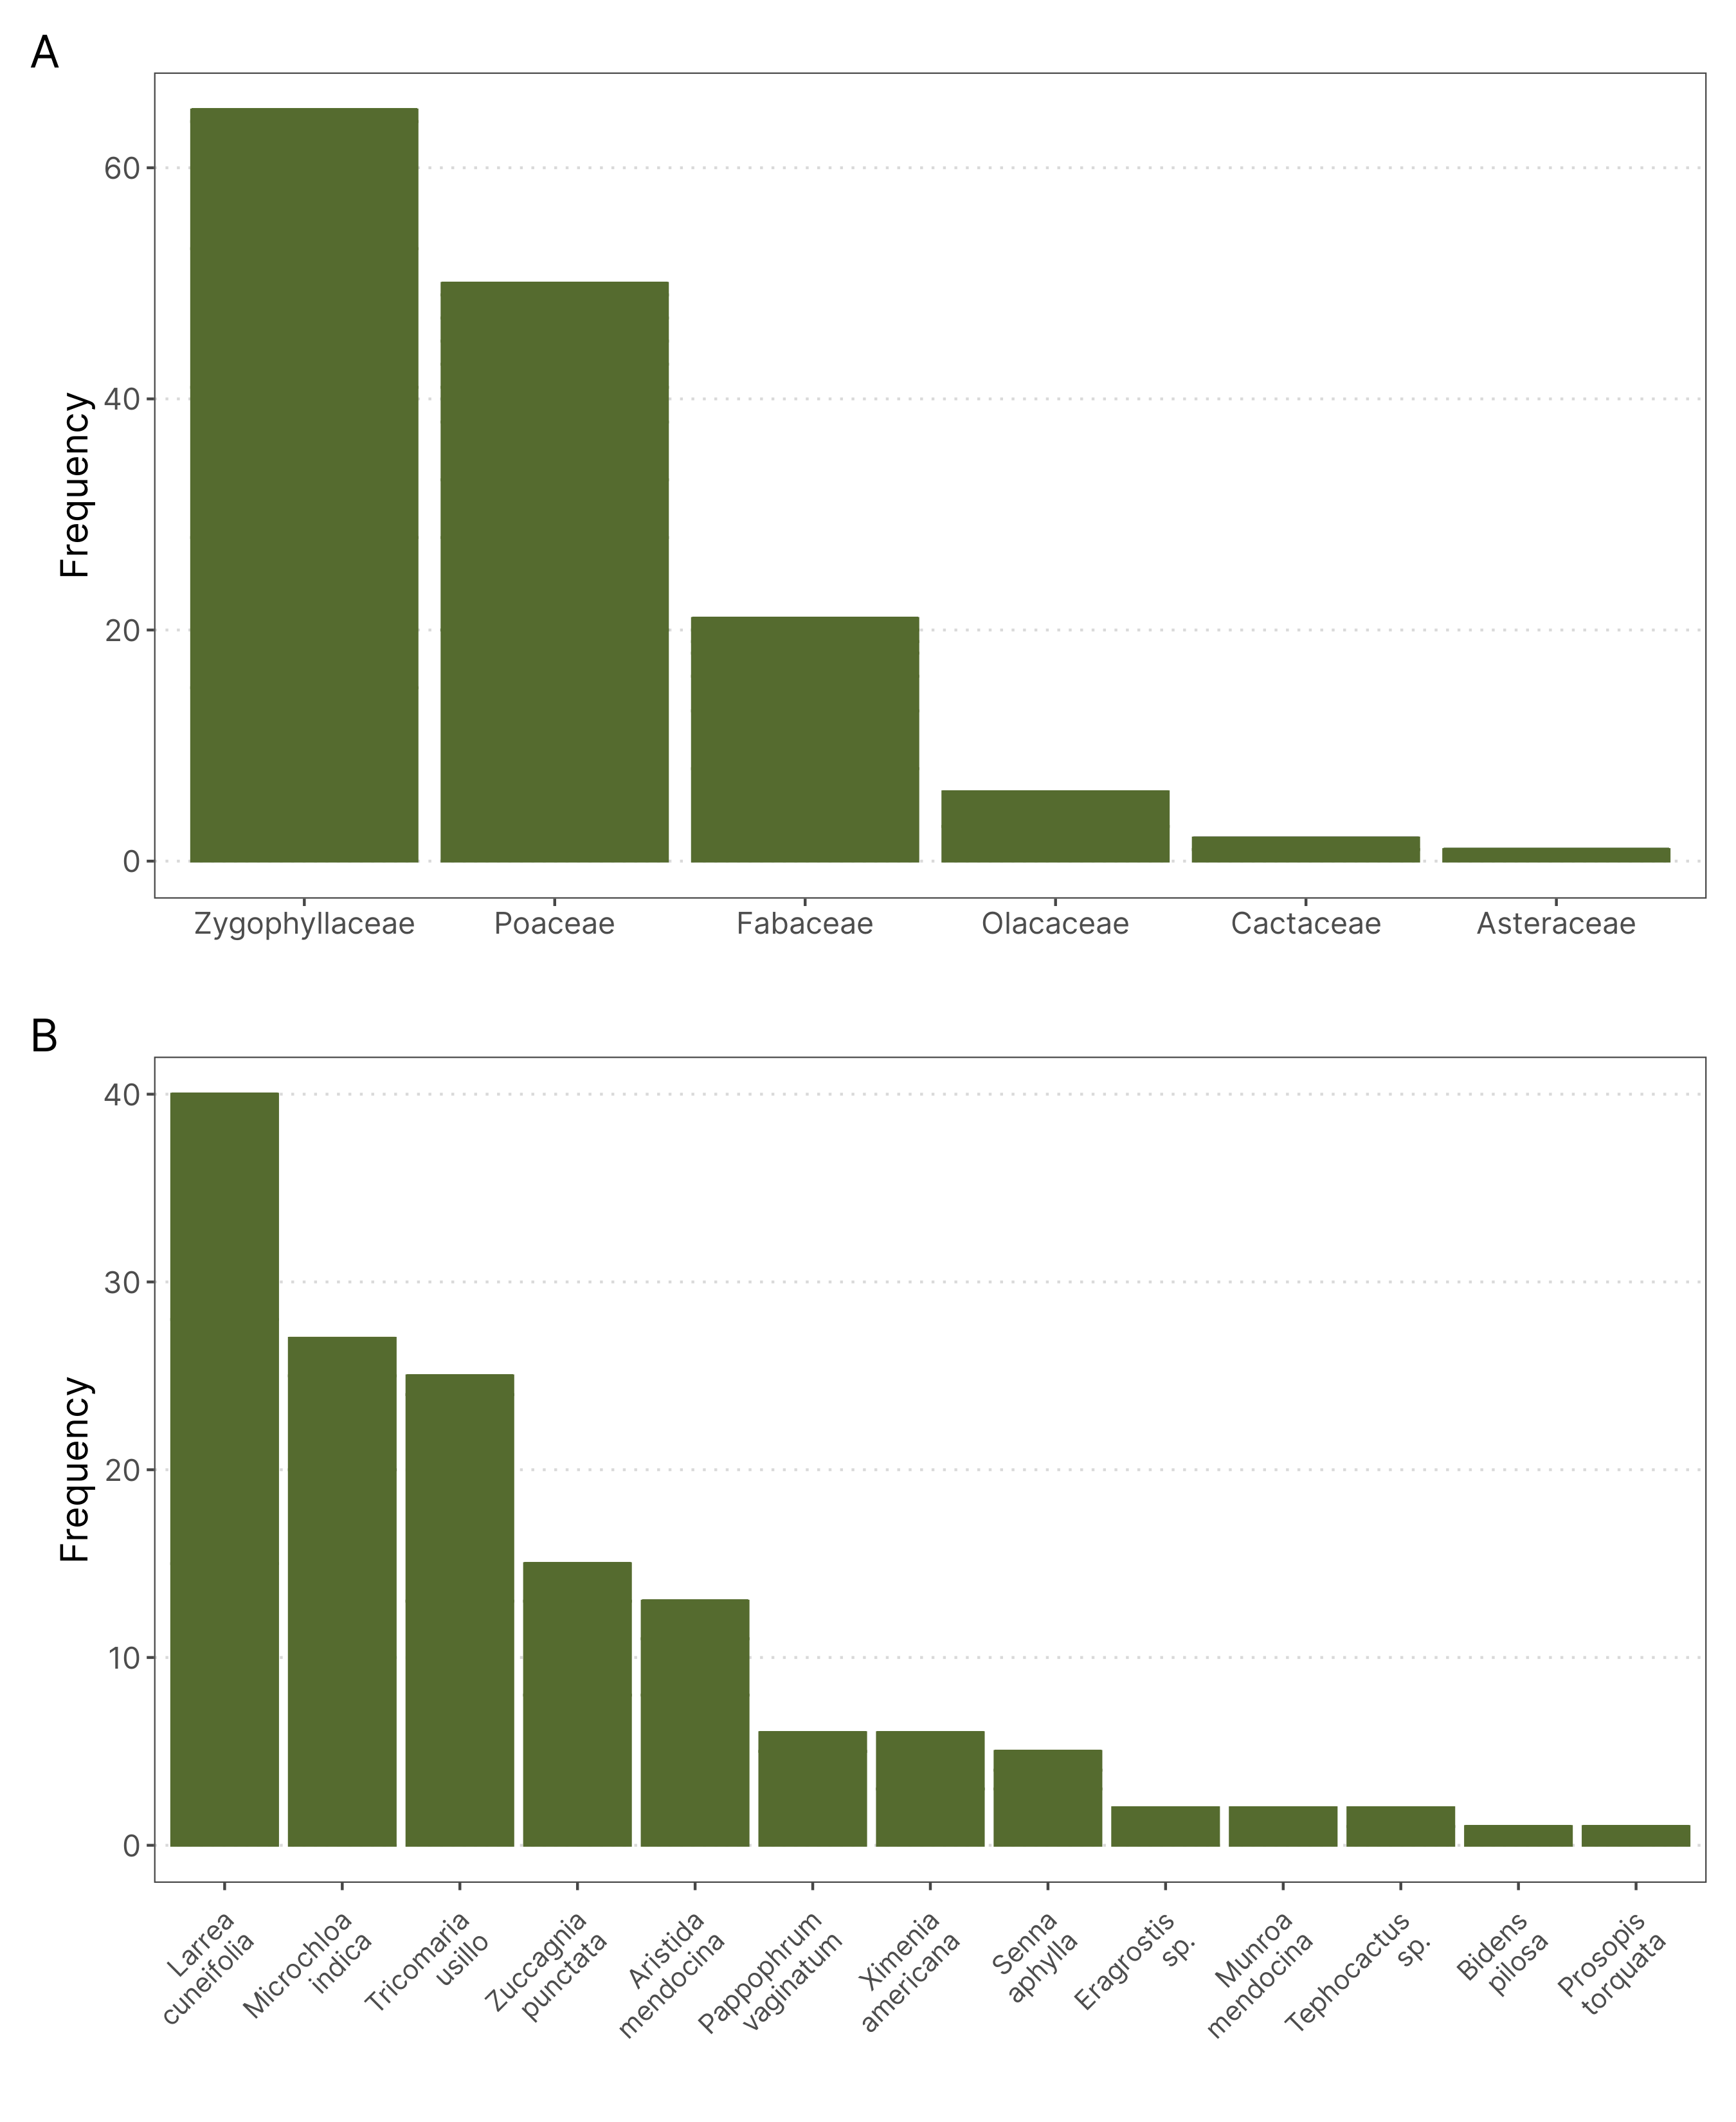
\includegraphics[width=1\linewidth]{../04_figures/appendix/plot_plants} 

  }

  \caption{Relative frequency of plants family (A) and species (B) in three transects near the Study Site. The plant community is dominated by members of the Zygolhyllaceae, Poaceae and Fabaceae families and is in accordance with what has been described in the literature. (n = 145)}\label{fig:appendix-plants}
  \end{figure}
  \hypertarget{anillacos-weather}{%
  \chapter{Anillaco's Weather}\label{anillacos-weather}}
  \begin{figure}

  {\centering 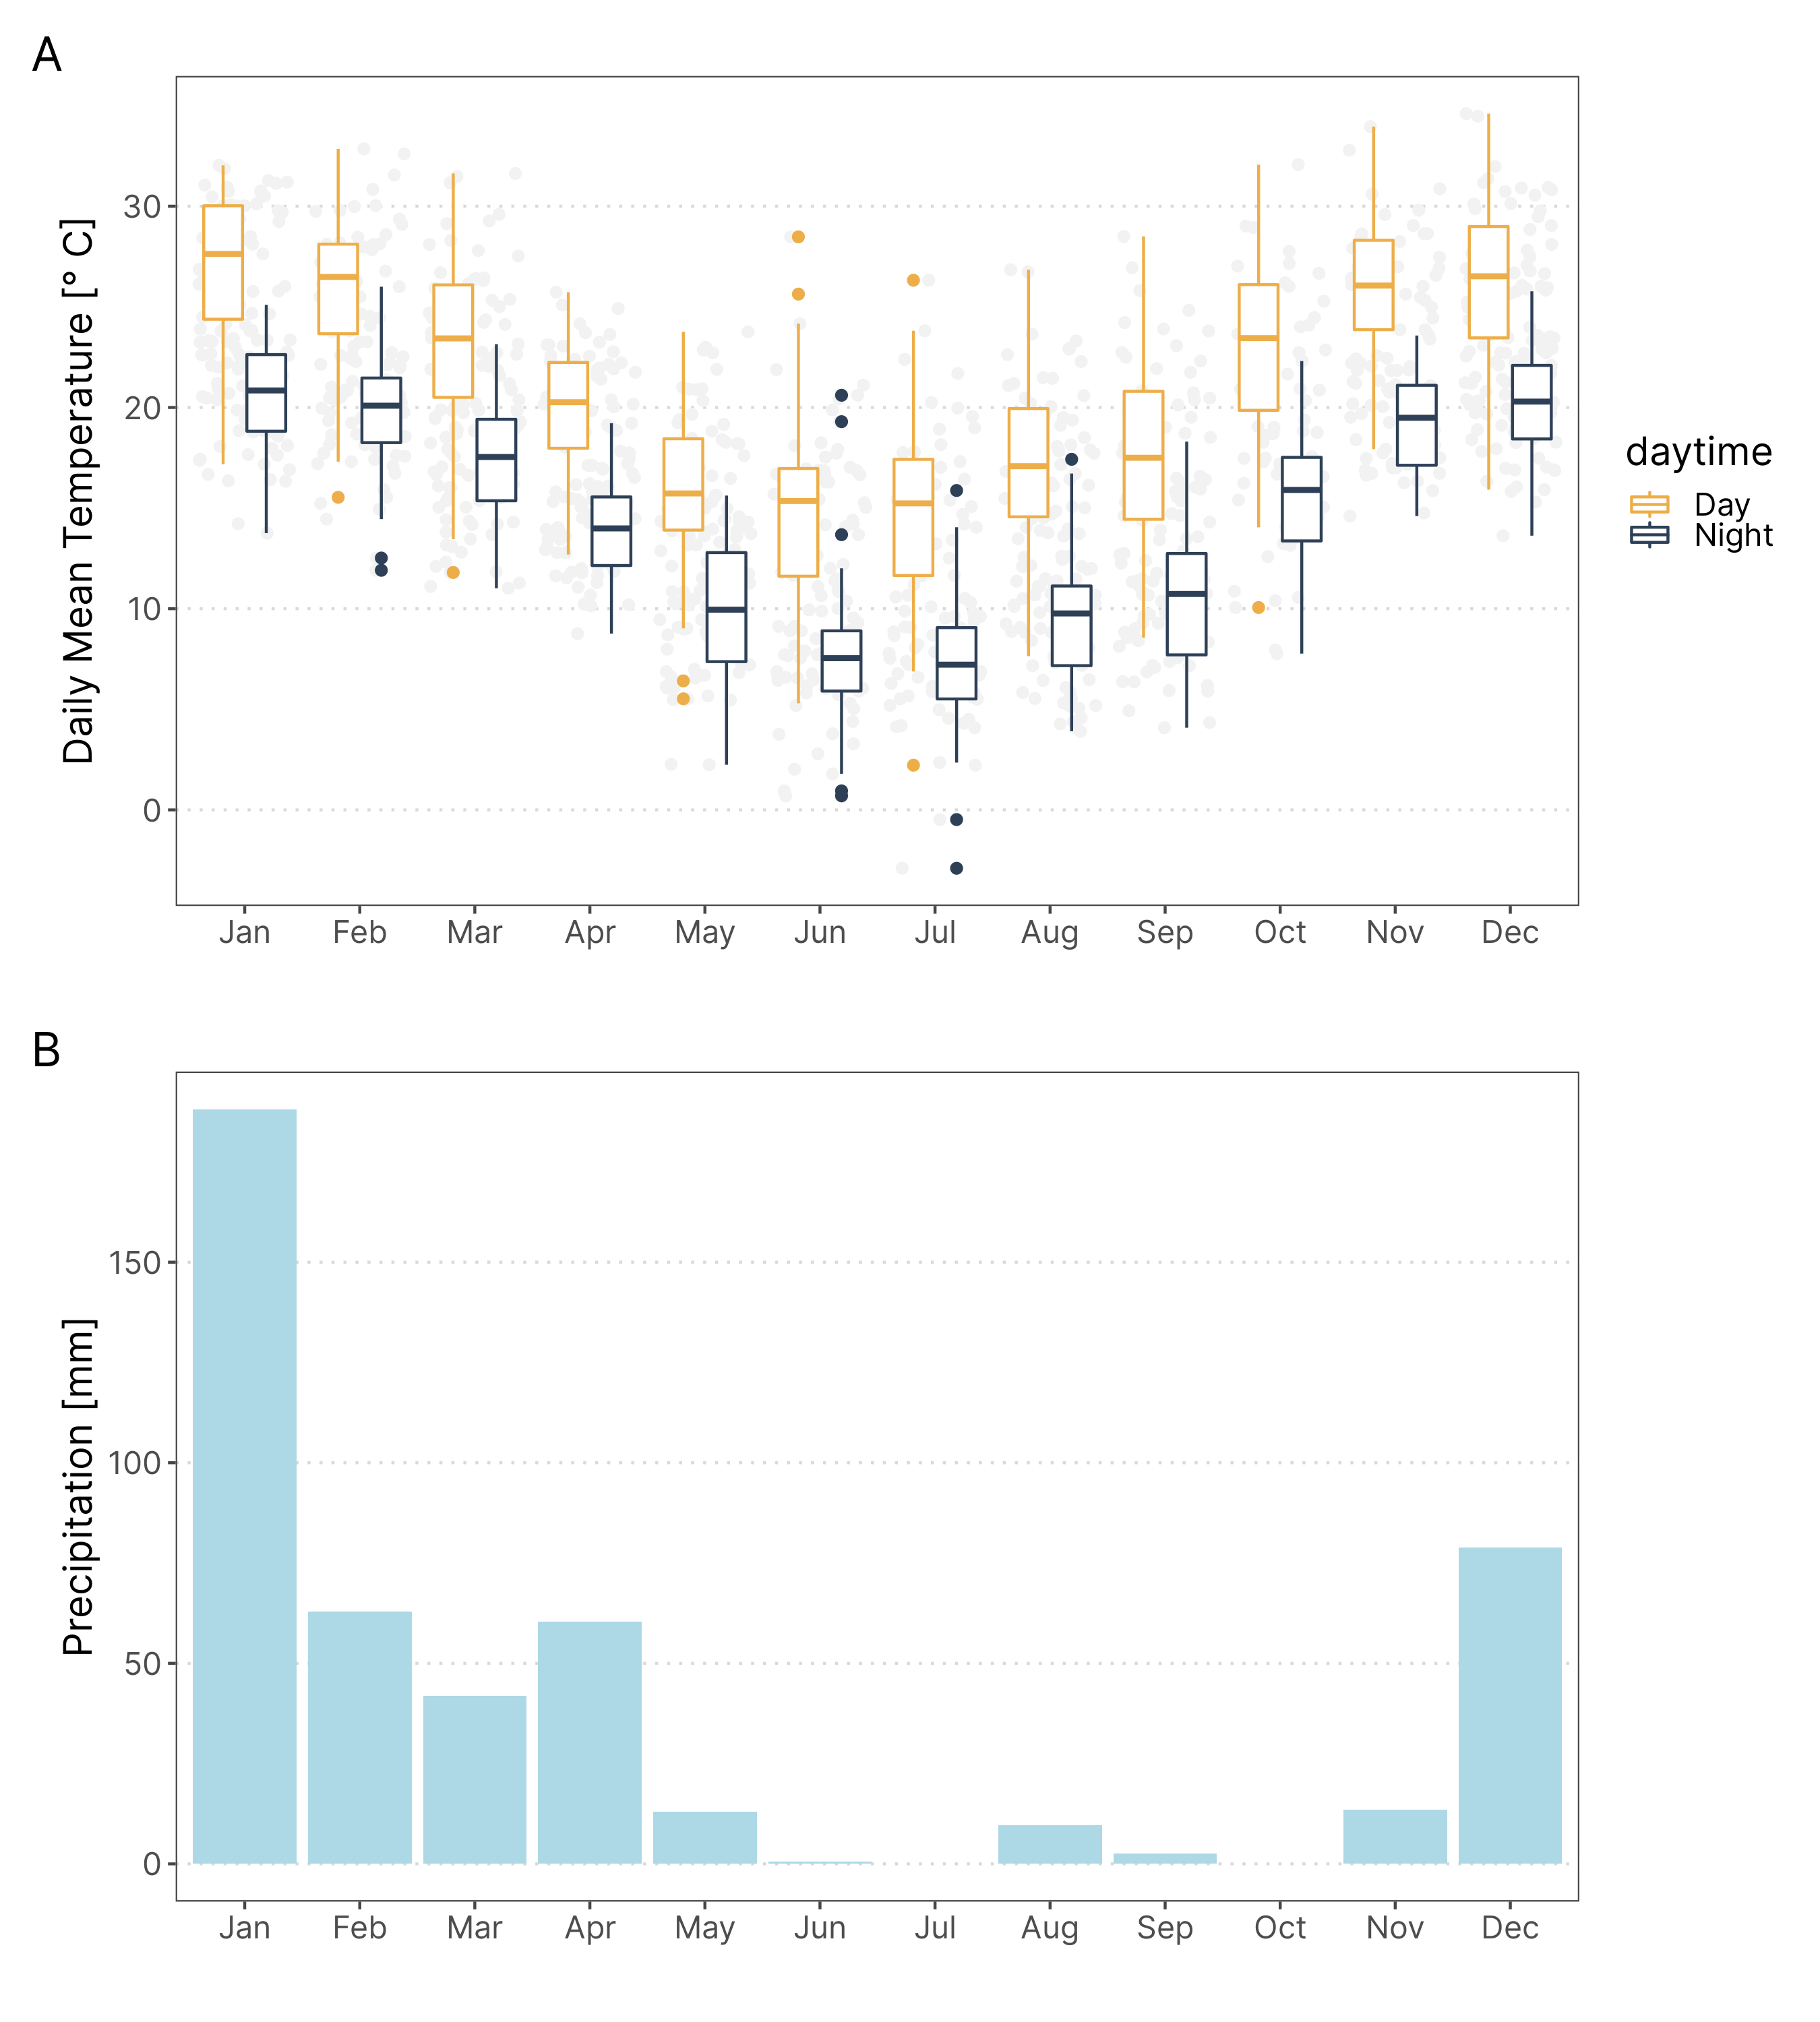
\includegraphics[width=1\linewidth]{../04_figures/appendix/plot_weather} 

  }

  \caption{Temperature  and Rainfall yearly trends in Anillaco, Argentina. Data was collected in the years 2017 and 2019 from a weather Station (Vantage Pro 2, Davis Instuments. USA.) maintened in CRILAR, aproximately 5km away from the study site.}\label{fig:appendix-weather}
  \end{figure}
  \hypertarget{anillacos-yearly-daylength-changes}{%
  \chapter{Anillaco's Yearly Daylength Changes}\label{anillacos-yearly-daylength-changes}}
  \begin{itemize}
  \tightlist
  \item
    Adicionar tabela com duração do dia nas datas de coleta
  \end{itemize}
  \begin{figure}

  {\centering 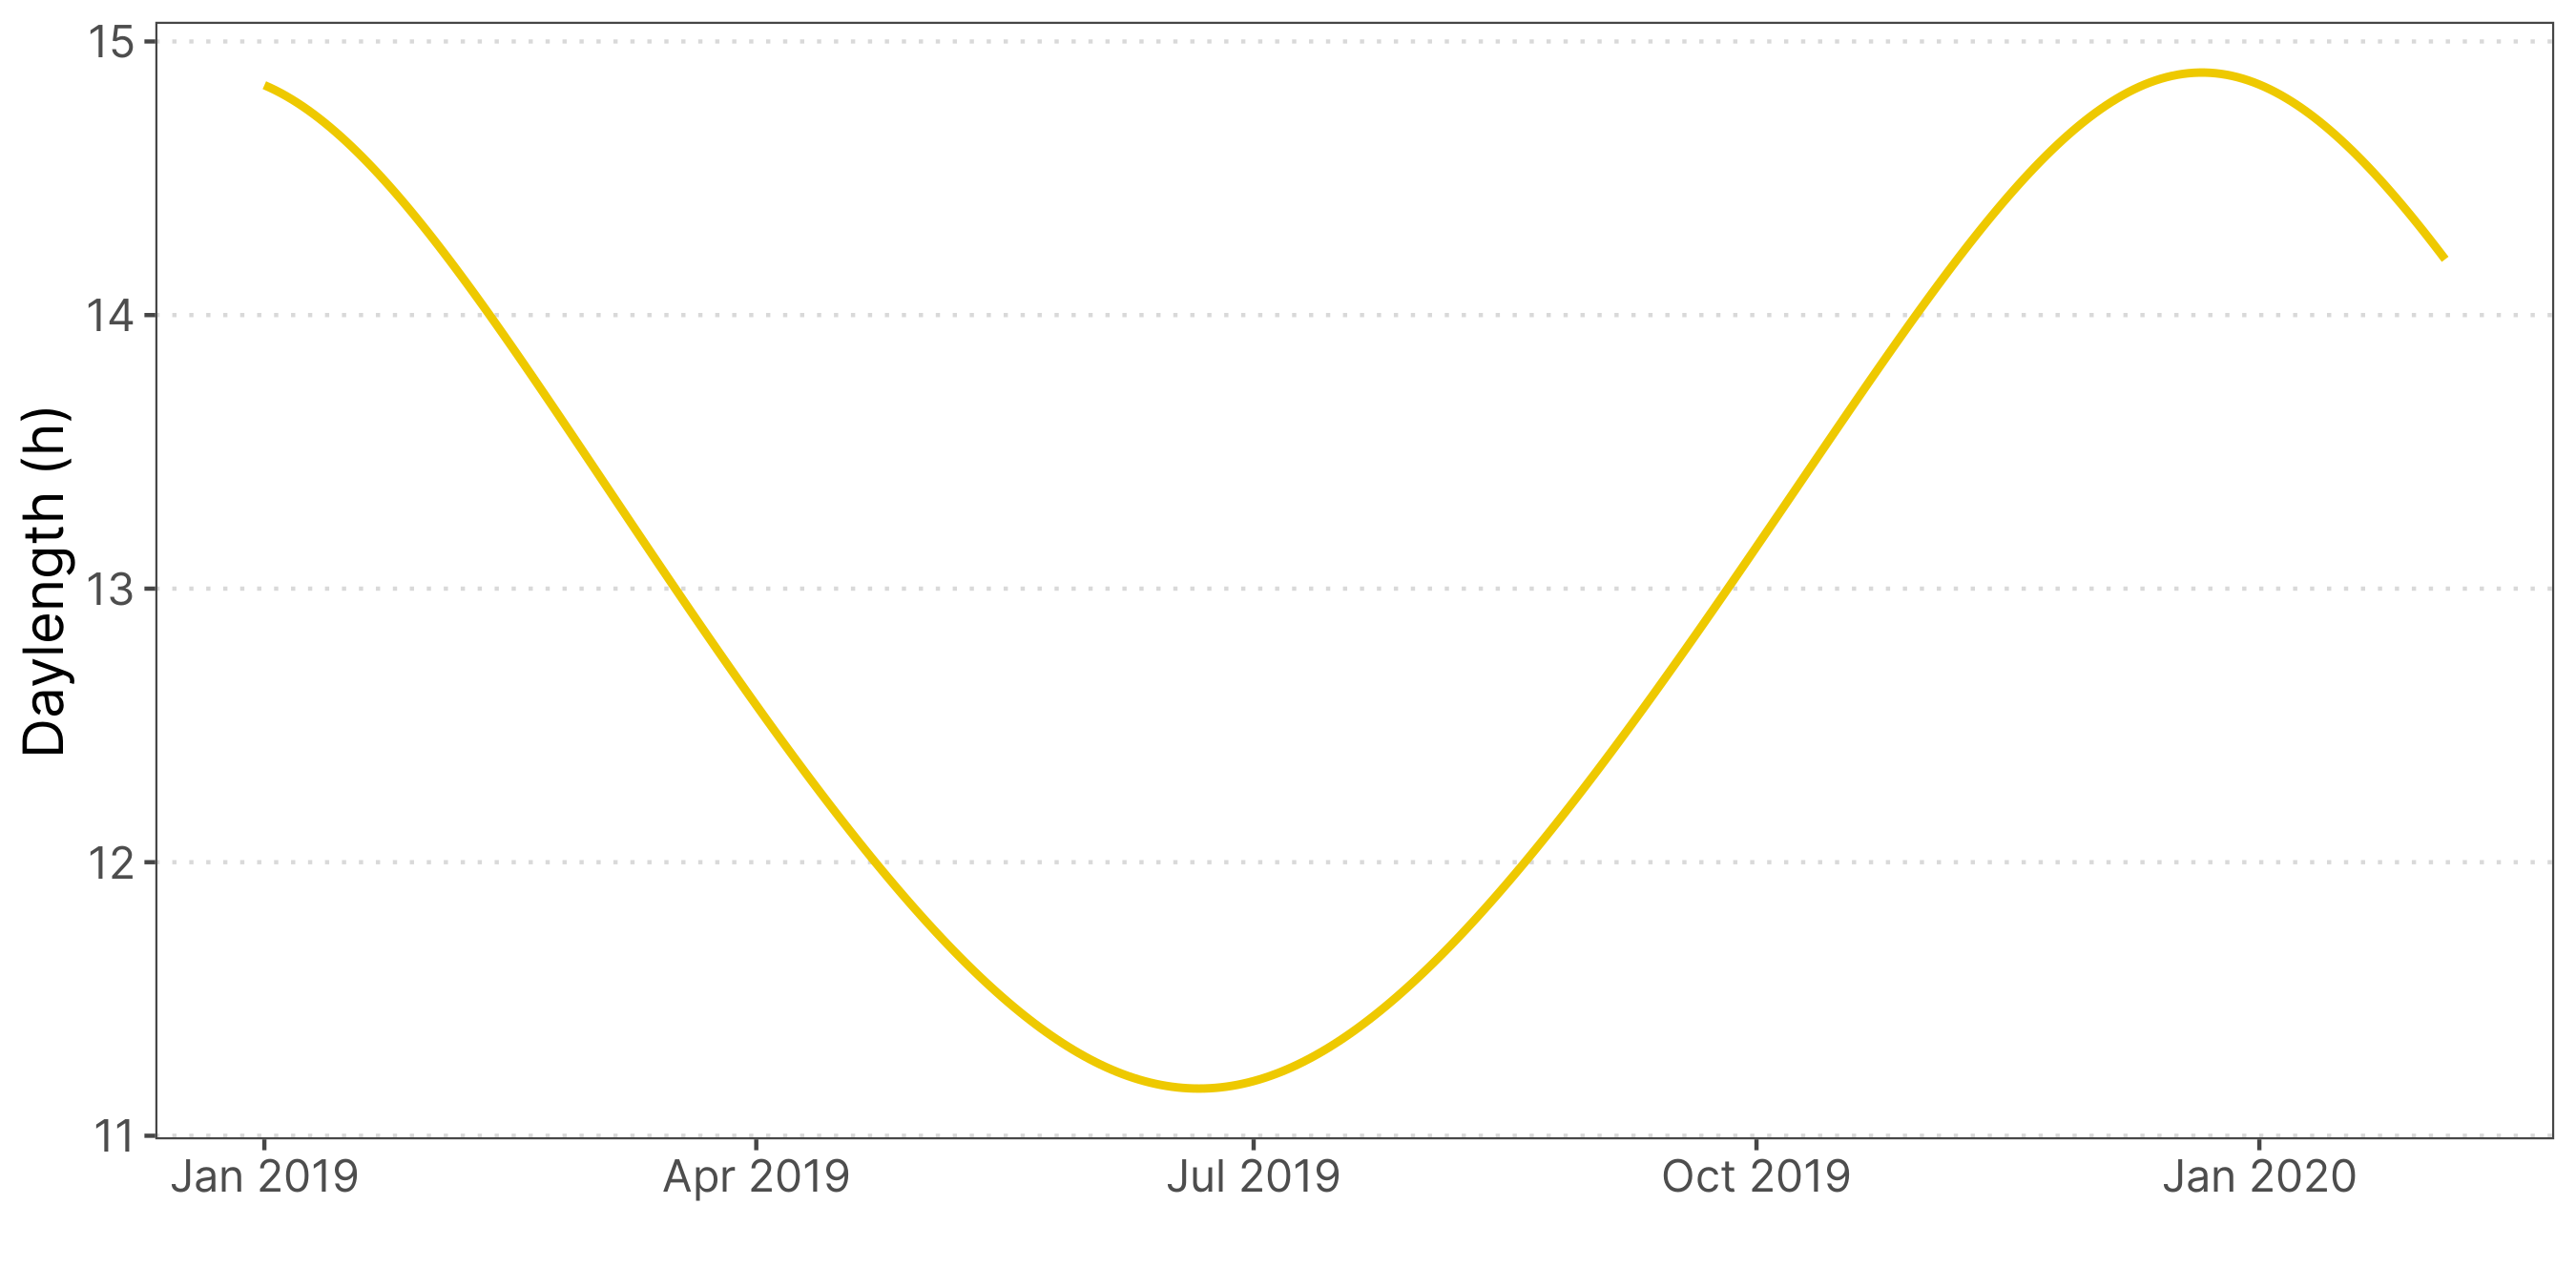
\includegraphics[width=1\linewidth]{../04_figures/appendix/plot_daylength} 

  }

  \caption{Changes in daytime changes across the year in Anillaco, La Rioja. Maximum duration of daytime, during summer, is 14 hours and 53 minutes. Mininum duration of daytime, during winter, is 11 hours and 10 minutes.}\label{fig:appendix-daylenght}
  \end{figure}
  \hypertarget{static-acceleration-smooth-window-assessment}{%
  \chapter{Static Acceleration Smooth Window Assessment}\label{static-acceleration-smooth-window-assessment}}

  \newpage
  \begin{center}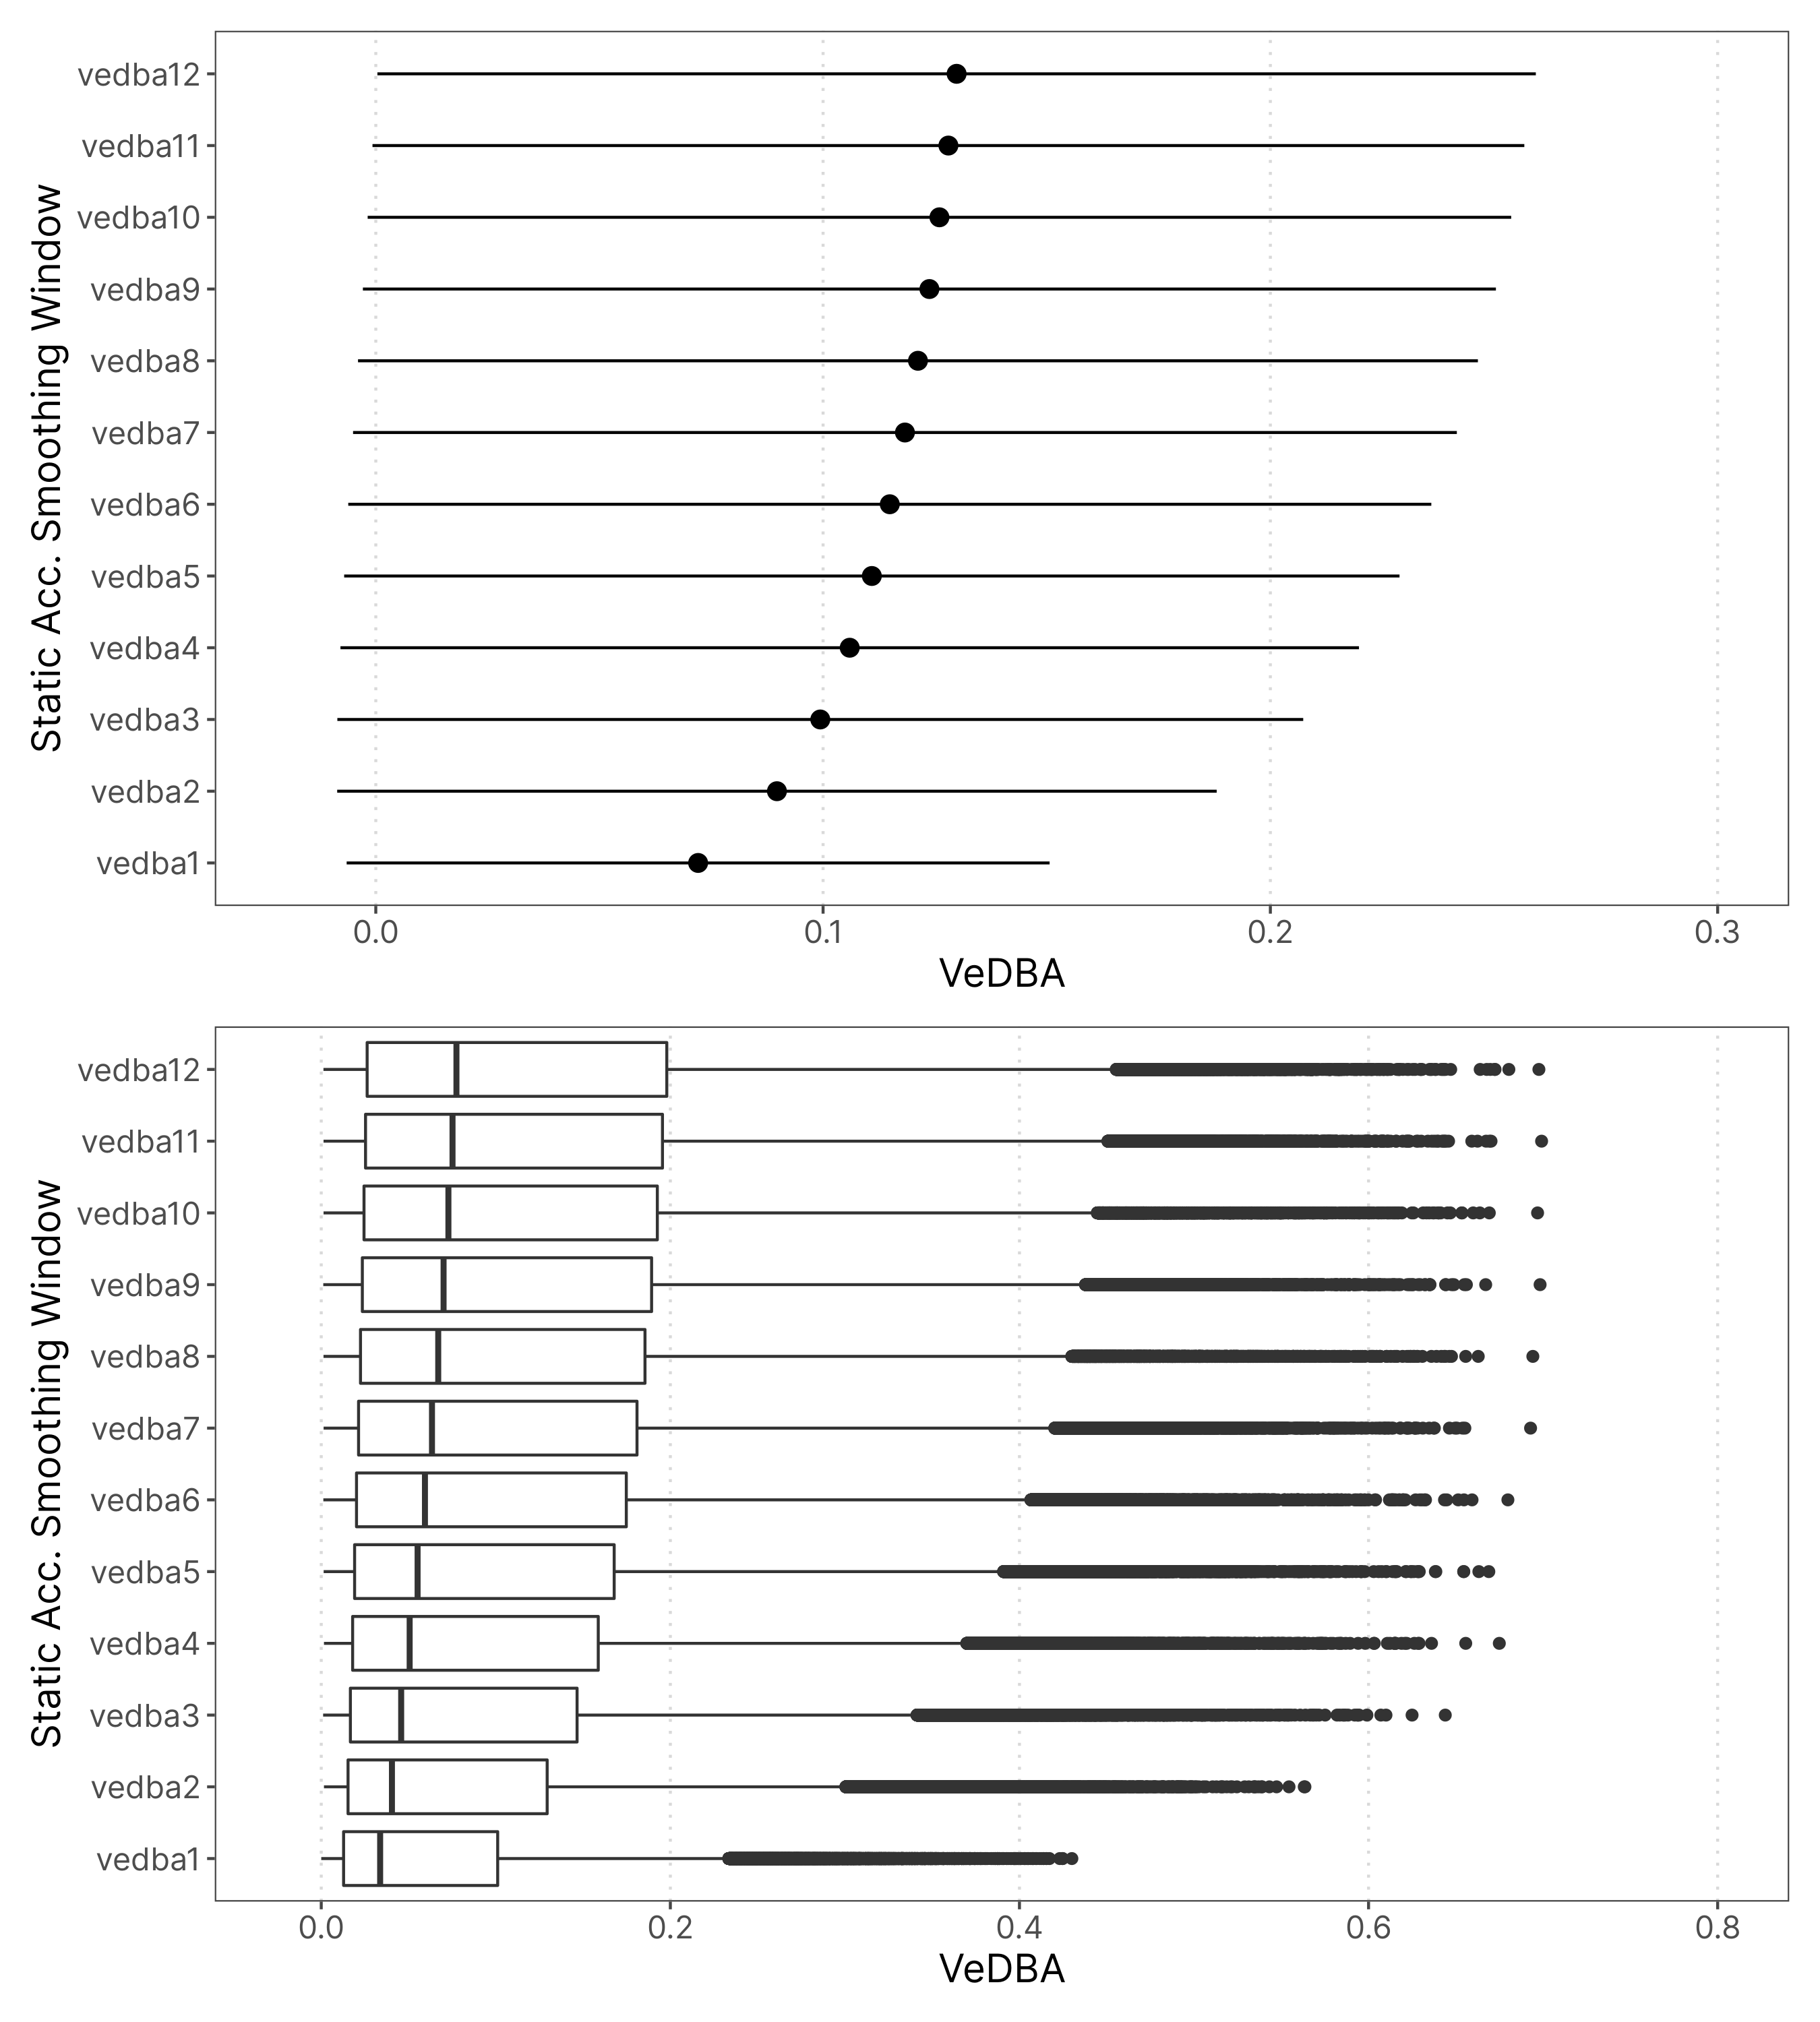
\includegraphics[width=1\linewidth]{../04_figures/appendix/plot_smoothing_window} \end{center}

  \hypertarget{exploratory-vedba-data-analysis}{%
  \chapter{Exploratory VeDBA data Analysis}\label{exploratory-vedba-data-analysis}}
  \begin{itemize}
  \tightlist
  \item
    adicionar descrião dos animais
    \begin{itemize}
    \tightlist
    \item
      peso, por sexo e estacao
    \end{itemize}
  \end{itemize}
  \hypertarget{time-series-plot}{%
  \section{Time Series Plot}\label{time-series-plot}}

  Primeiro uma verificada geral nos dados em formato de série temporal. Os gráficos mostram apenas os 4 primeiros dias de registro de cada animal.

  Não é possível ver muita diferença entre os animais então nas séries temporais então estão plotados apenas 4 animais. É interessante que em alguns animais já é possível ver que oo pontos parecem estar mais ou menos organizados em três regiões distintas na vertical.
  \begin{center}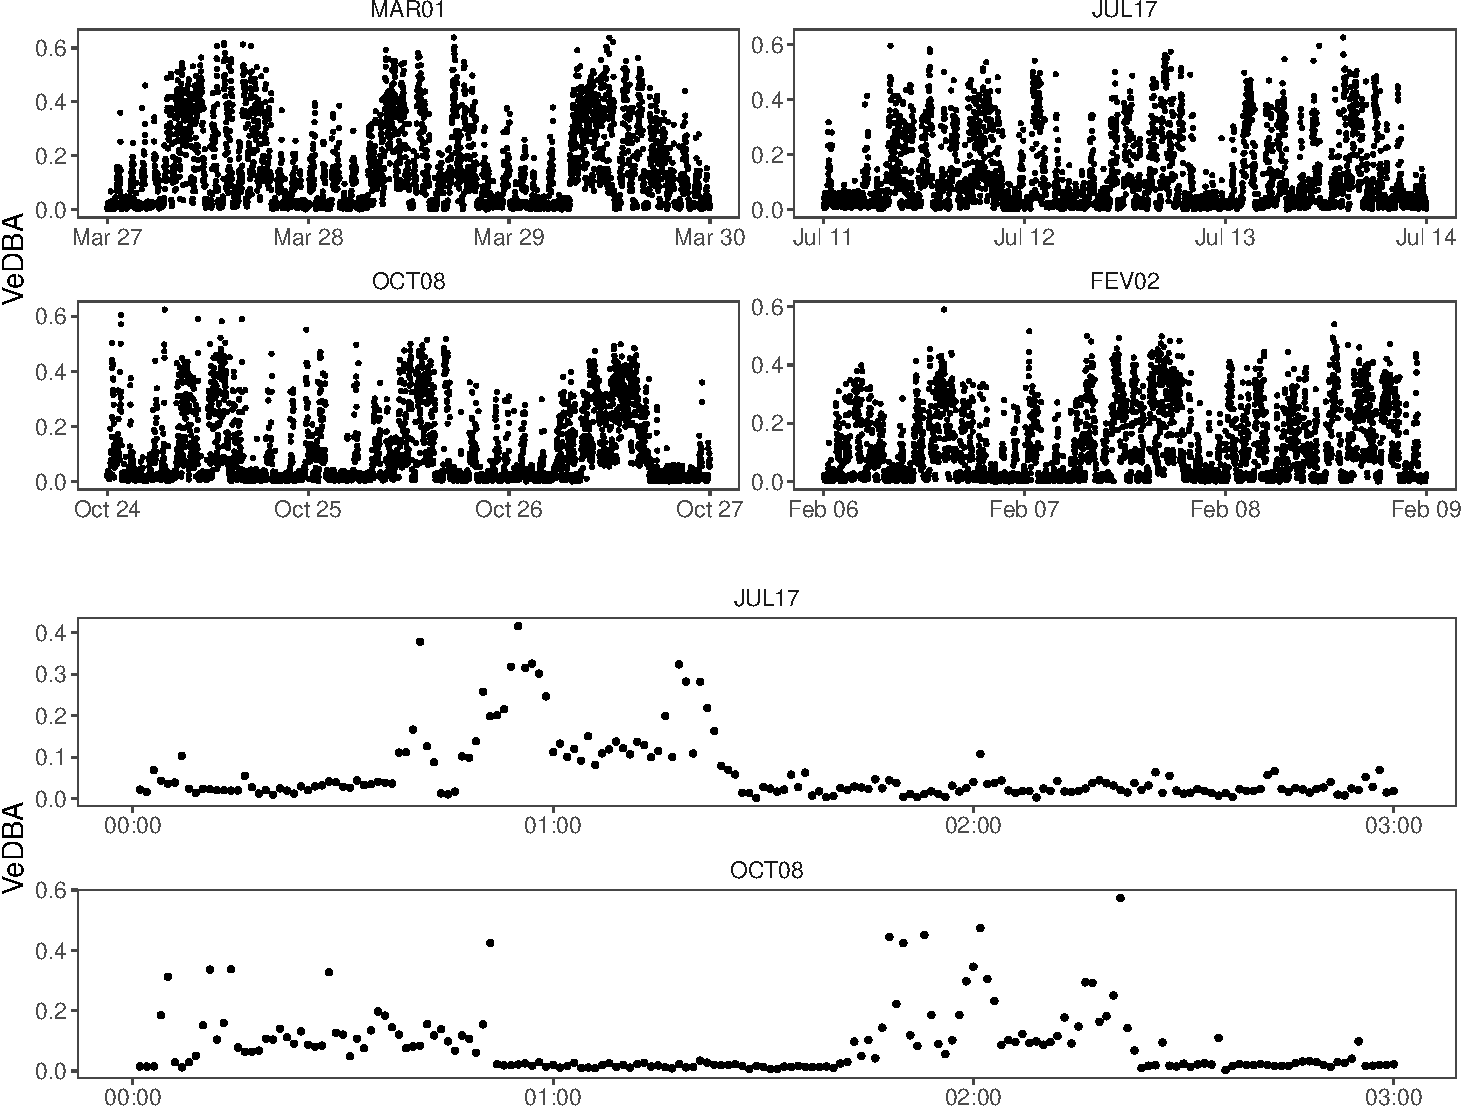
\includegraphics[width=1\linewidth]{tese_jefferson_files/figure-latex/timeseries-1} \end{center}

  \newpage

  \hypertarget{histogramas-e-gruxe1ficos-de-densidade}{%
  \section{Histogramas e Gráficos de Densidade}\label{histogramas-e-gruxe1ficos-de-densidade}}

  Antes de seguir para outras análises vamos observar as distribuições dos dados de acelerômetros para ver se há muita heterogeneidade entre os animais. Os dados de atividade para esses gráficos foram limitados à 4 dias por animal, assim o número de amostras por animal é o mesmo.

  As distribuições de VeDBA parecem ter um range muito próximo de valores. Ou seja, parece não haver animais que possuam uma atividade muito mais intensa do que outros, o que também pode ser visto na tabela abaixo. Porém, o formato da distribuição muda entre alguns animais, principalmente entre estações. Por exemplo, os animais capturados em outubro parecem ter maior número de amostras com valores mais à direita da distribuição, entre 0.2 e 0.5. Alguns animais capturados em Fevereiro parecem continuar com essa tendência. Em julho, porém, os animais parecem ter uma distribuição com maior concentração em valores mais centrais, entre 0.05 e 0.2. Essas mesmas tendências também podem ser observadas de uma forma mais compacta no gráficos de densidade por animal.

  Então, os animais, apesar de terem distribuição de VeDBA que não distoam muito uns dos outros no seu range, parecem passar tempos diferentes em tipos de diferentes de comportamentos.

  \newpage
  \begin{table}[!h]
  \centering
  \begin{tabular}{cccccccc}
  \toprule
  ID & season & Mean & Median & Max & Min & Range & VeDBA\_Sum\\
  \midrule
  MAR01 & March & 0.145 & 0.097 & 0.639 & 0.001 & 0.638 & 624.996\\
  MAR02 & March & 0.115 & 0.055 & 0.728 & 0.001 & 0.727 & 494.680\\
  JUL15 & July & 0.123 & 0.079 & 0.755 & 0.000 & 0.755 & 532.374\\
  JUL16 & July & 0.091 & 0.030 & 0.740 & 0.002 & 0.738 & 393.167\\
  JUL17 & July & 0.109 & 0.042 & 0.627 & 0.000 & 0.627 & 471.670\\
  \addlinespace
  JUL18 & July & 0.096 & 0.034 & 0.623 & 0.000 & 0.623 & 413.211\\
  JUL19 & July & 0.101 & 0.075 & 0.641 & 0.001 & 0.641 & 435.153\\
  JUL20 & July & 0.091 & 0.063 & 0.624 & 0.000 & 0.624 & 395.131\\
  JUL21 & July & 0.112 & 0.056 & 0.609 & 0.001 & 0.608 & 485.622\\
  JUL23 & July & 0.114 & 0.047 & 0.711 & 0.001 & 0.710 & 491.648\\
  \addlinespace
  OCT01 & October & 0.111 & 0.056 & 0.672 & 0.007 & 0.665 & 477.646\\
  OCT08 & October & 0.102 & 0.036 & 0.624 & 0.000 & 0.624 & 439.019\\
  OCT09 & October & 0.167 & 0.099 & 0.657 & 0.001 & 0.656 & 722.404\\
  OCT10 & October & 0.147 & 0.089 & 0.593 & 0.000 & 0.593 & 635.926\\
  OCT13 & October & 0.126 & 0.064 & 0.540 & 0.001 & 0.539 & 542.222\\
  \addlinespace
  OCT14 & October & 0.130 & 0.066 & 0.555 & 0.007 & 0.548 & 563.757\\
  FEV01 & February & 0.138 & 0.089 & 0.629 & 0.000 & 0.629 & 594.794\\
  FEV02 & February & 0.113 & 0.072 & 0.590 & 0.000 & 0.590 & 488.959\\
  FEV03 & February & 0.103 & 0.072 & 0.654 & 0.000 & 0.654 & 445.102\\
  FEV05 & February & 0.119 & 0.049 & 0.601 & 0.007 & 0.594 & 514.446\\
  \addlinespace
  FEV06 & February & 0.129 & 0.069 & 0.577 & 0.002 & 0.576 & 557.528\\
  \bottomrule
  \end{tabular}
  \end{table}
  \newpage
  \begin{figure}[H]

  {\centering 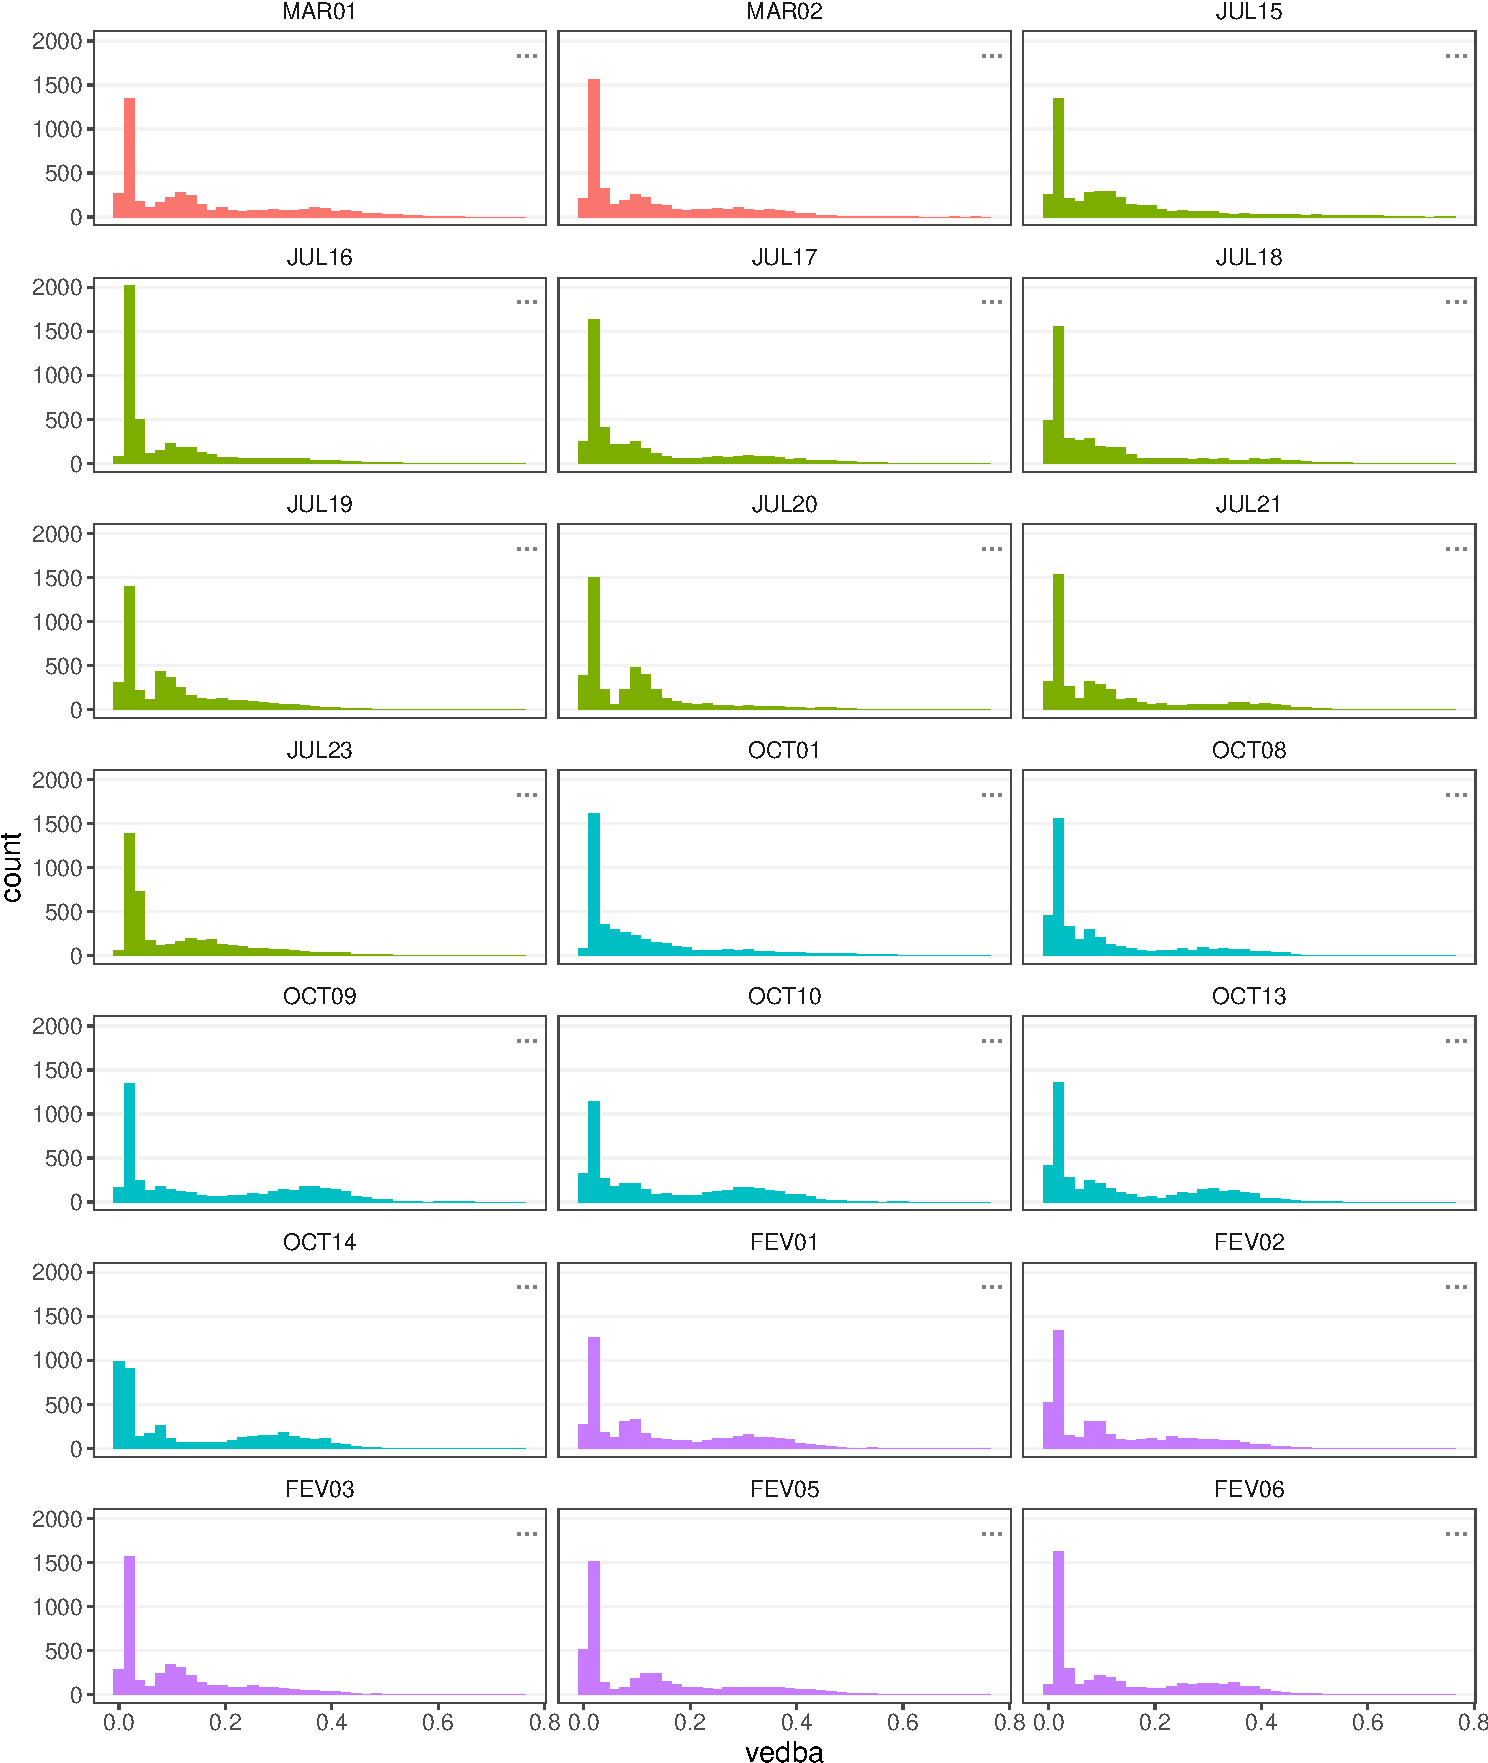
\includegraphics[width=1\linewidth]{tese_jefferson_files/figure-latex/hist-1} 

  }

  \caption{Histograma dos valore de VeDBA por animal (cada quadro). As cores representam os meses em que esses animais foram capturados.}\label{fig:hist}
  \end{figure}
  \newpage
  \begin{figure}[H]

  {\centering 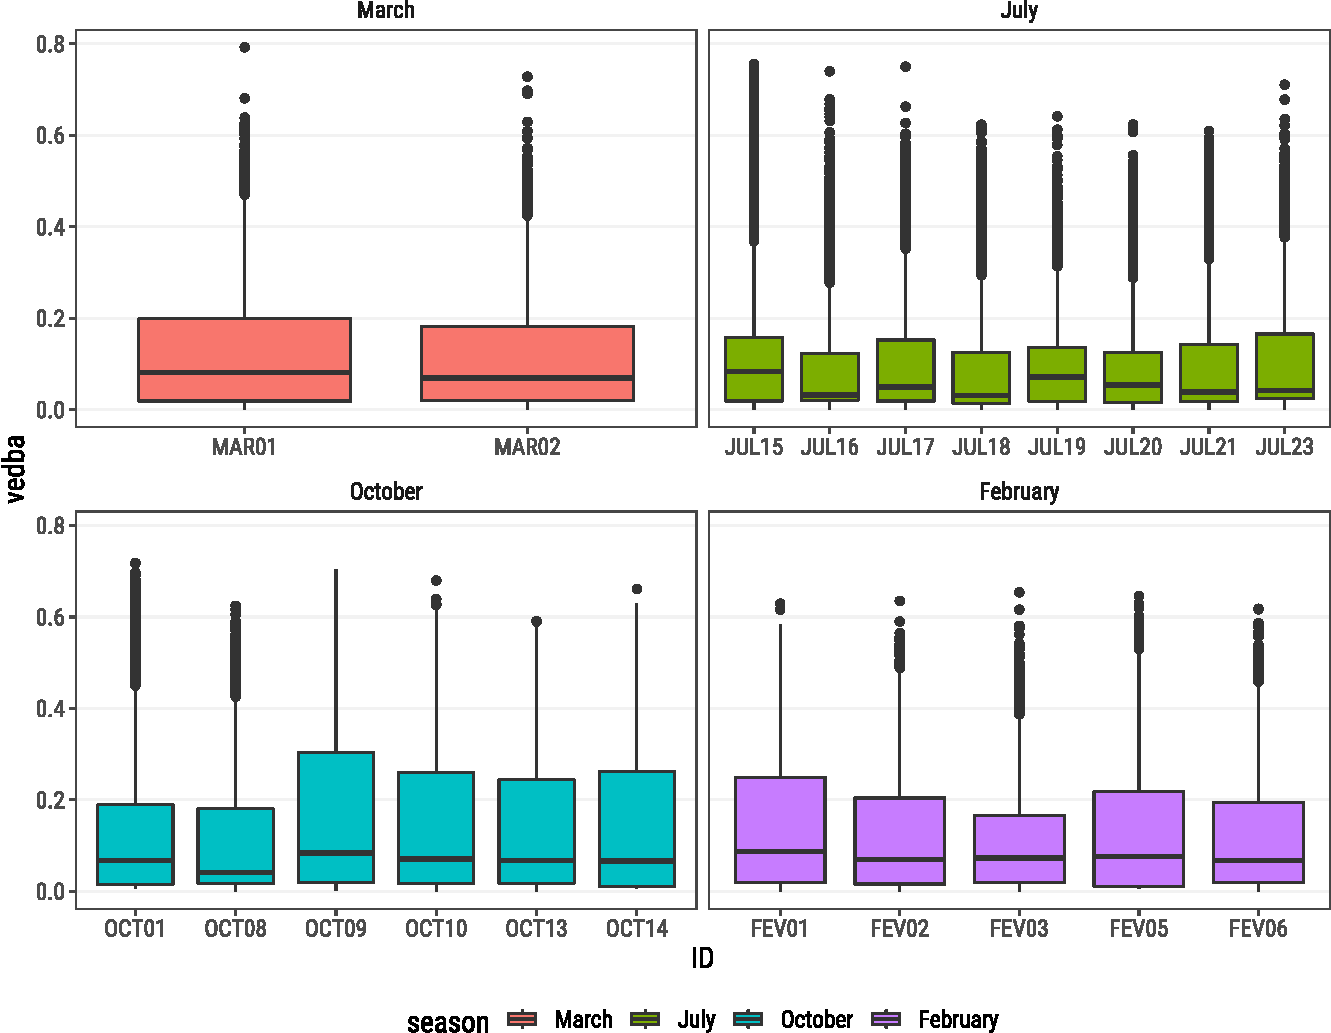
\includegraphics[width=1\linewidth]{tese_jefferson_files/figure-latex/boxplot-1} 

  }

  \caption{Ridge plot mostrando a densidade da distribuição dos valores de VeDBA divididos por animal. As cores representam os meses em que os animais foram capturados.}\label{fig:boxplot}
  \end{figure}
  \newpage

  \hypertarget{padruxf5es-muxe9dios-de-atividade-por-animal}{%
  \section{Padrões Médios de Atividade por Animal}\label{padruxf5es-muxe9dios-de-atividade-por-animal}}

  Para terminar, é interessante ver como é o ``ritmo médio'' ao longo de todo tempo de registro dos animais. Acho que esse gráfico é especialmente interessante para pessoas fora da cronobiologia, já que é bem mais intuitivo do que os actogramas.

  Nesses primeiro gráfico foi plotado a média por hora dos valores de VeDBA de cada animal.
  \begin{center}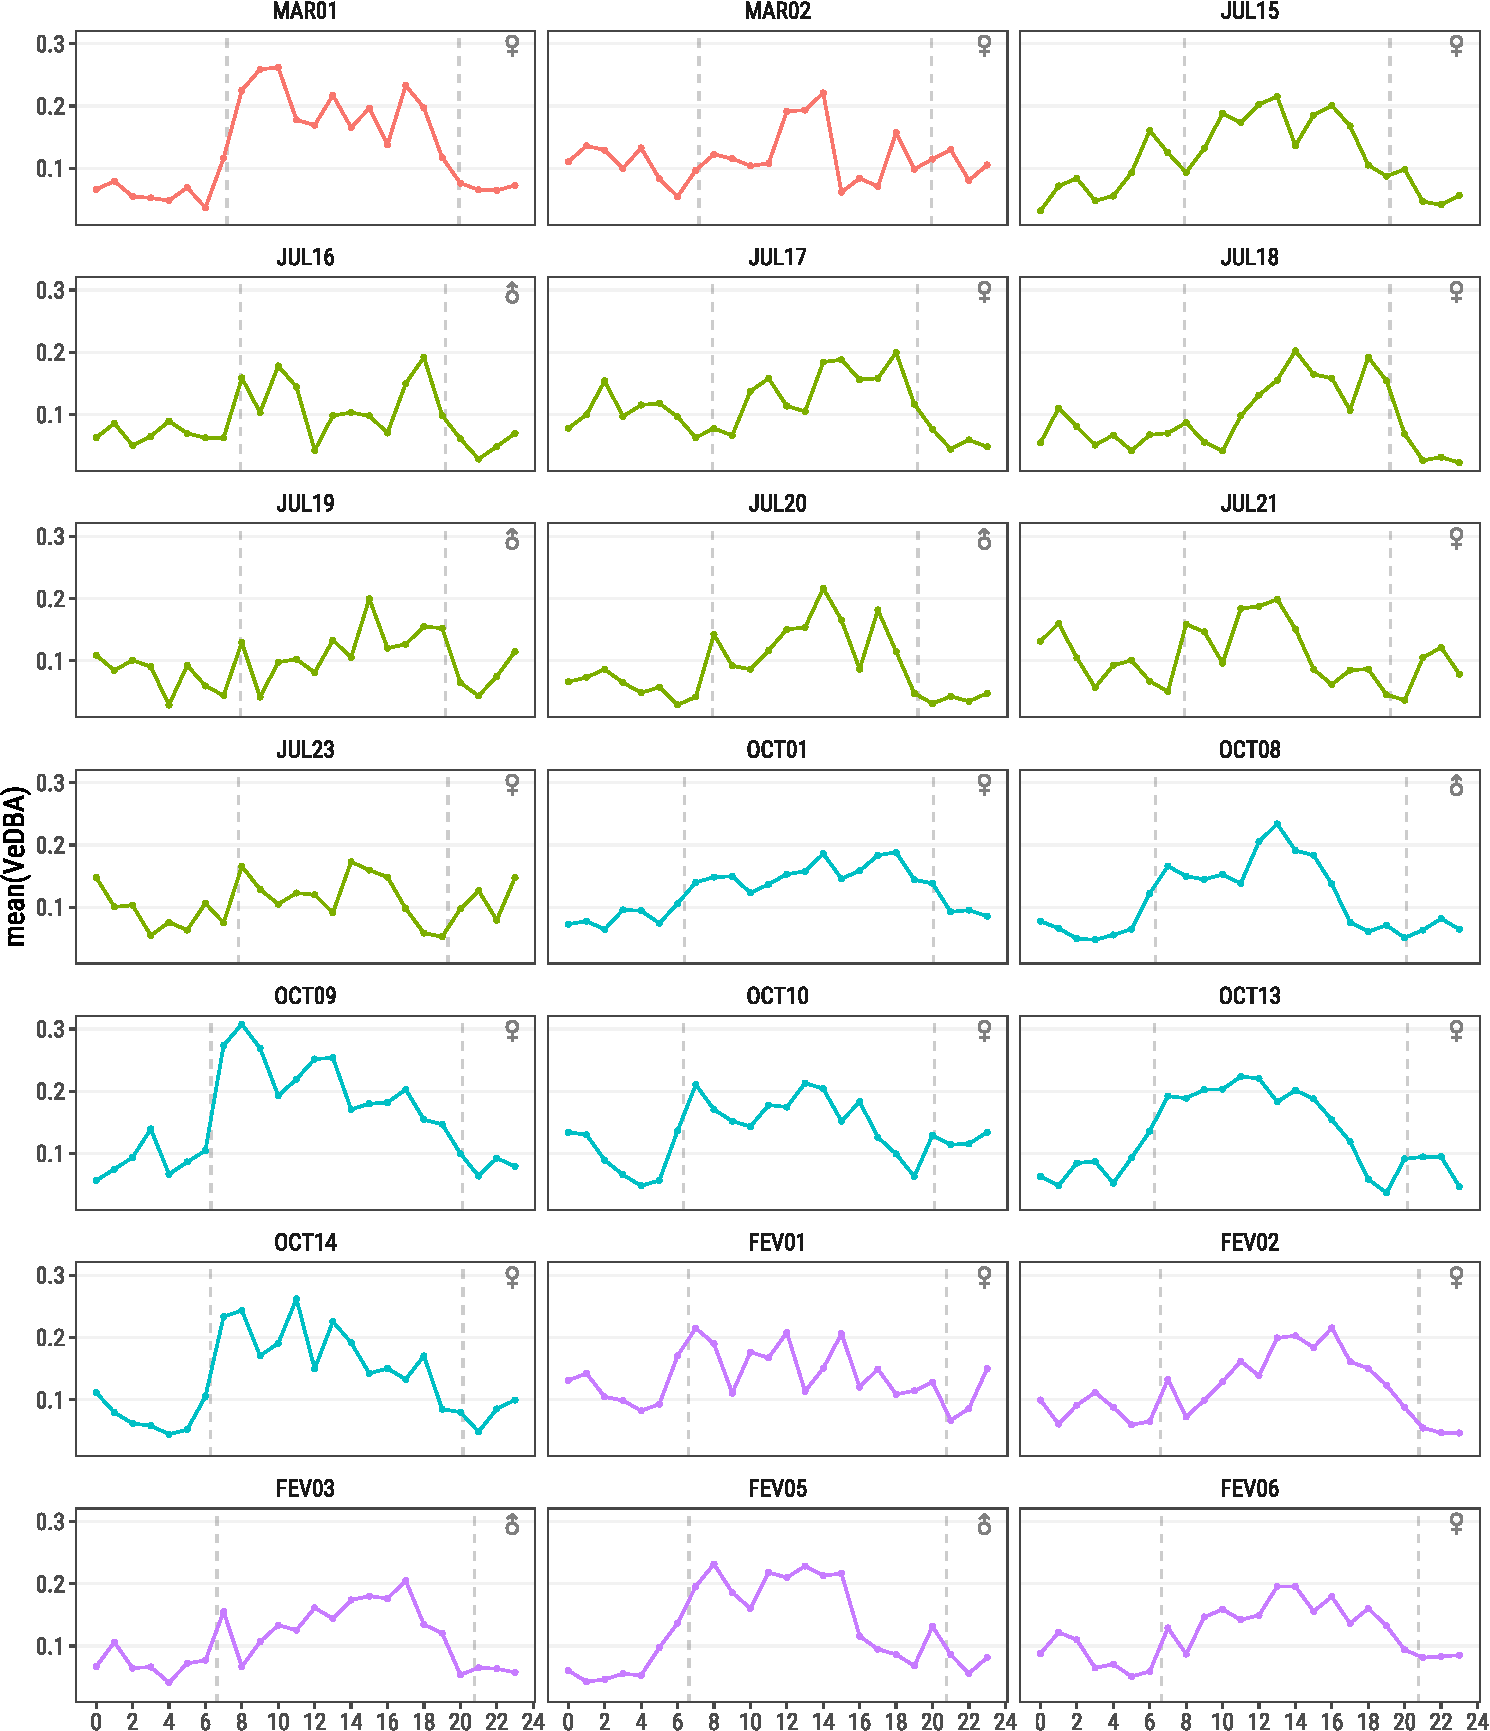
\includegraphics[width=1\linewidth]{tese_jefferson_files/figure-latex/graph-hourly-id-1} \end{center}

  \newpage

  \hypertarget{gruxe1ficos-agrupados-por-estauxe7uxe3o-e-sexo}{%
  \section{Gráficos Agrupados por Estação e Sexo}\label{gruxe1ficos-agrupados-por-estauxe7uxe3o-e-sexo}}

  \hypertarget{histogramasgruxe1fico-de-densidade}{%
  \subsection{Histogramas/Gráfico de Densidade}\label{histogramasgruxe1fico-de-densidade}}

  Visualmente parece haver alguma diferença sazonal nas atividade dos tucos. Vamos inspecionar melhor isso agrupando os dados por estação e sexo.

  Como o número de amostras varia entre estações e sexo o histograma não seria muito informativo nesse caso. Então pra isso podemos fazer um gráfico de densidade. Esses gráficos basicamente refletem a forma do histograma mas, nesse caso, tem a vantagem de que são padronizados para que a área abaixo da curva serja sempre igual a 1.

  Assim, podemos ver como o perfil das distribuições muda ao longo das estações e entre sexos mesmo tendo um número de amostras diferente para cada condição. Os valores em \texttt{y} não significam muita coisa individualmente.

  Visualmente temos o que também vimos nos histogramas anteriores. A distribuição parece mudar ao longo do ano. No entanto, quando sobrepomos as distribuições de cada sexo parece não haver muita diferença entre machos e fêmeas.
  \begin{center}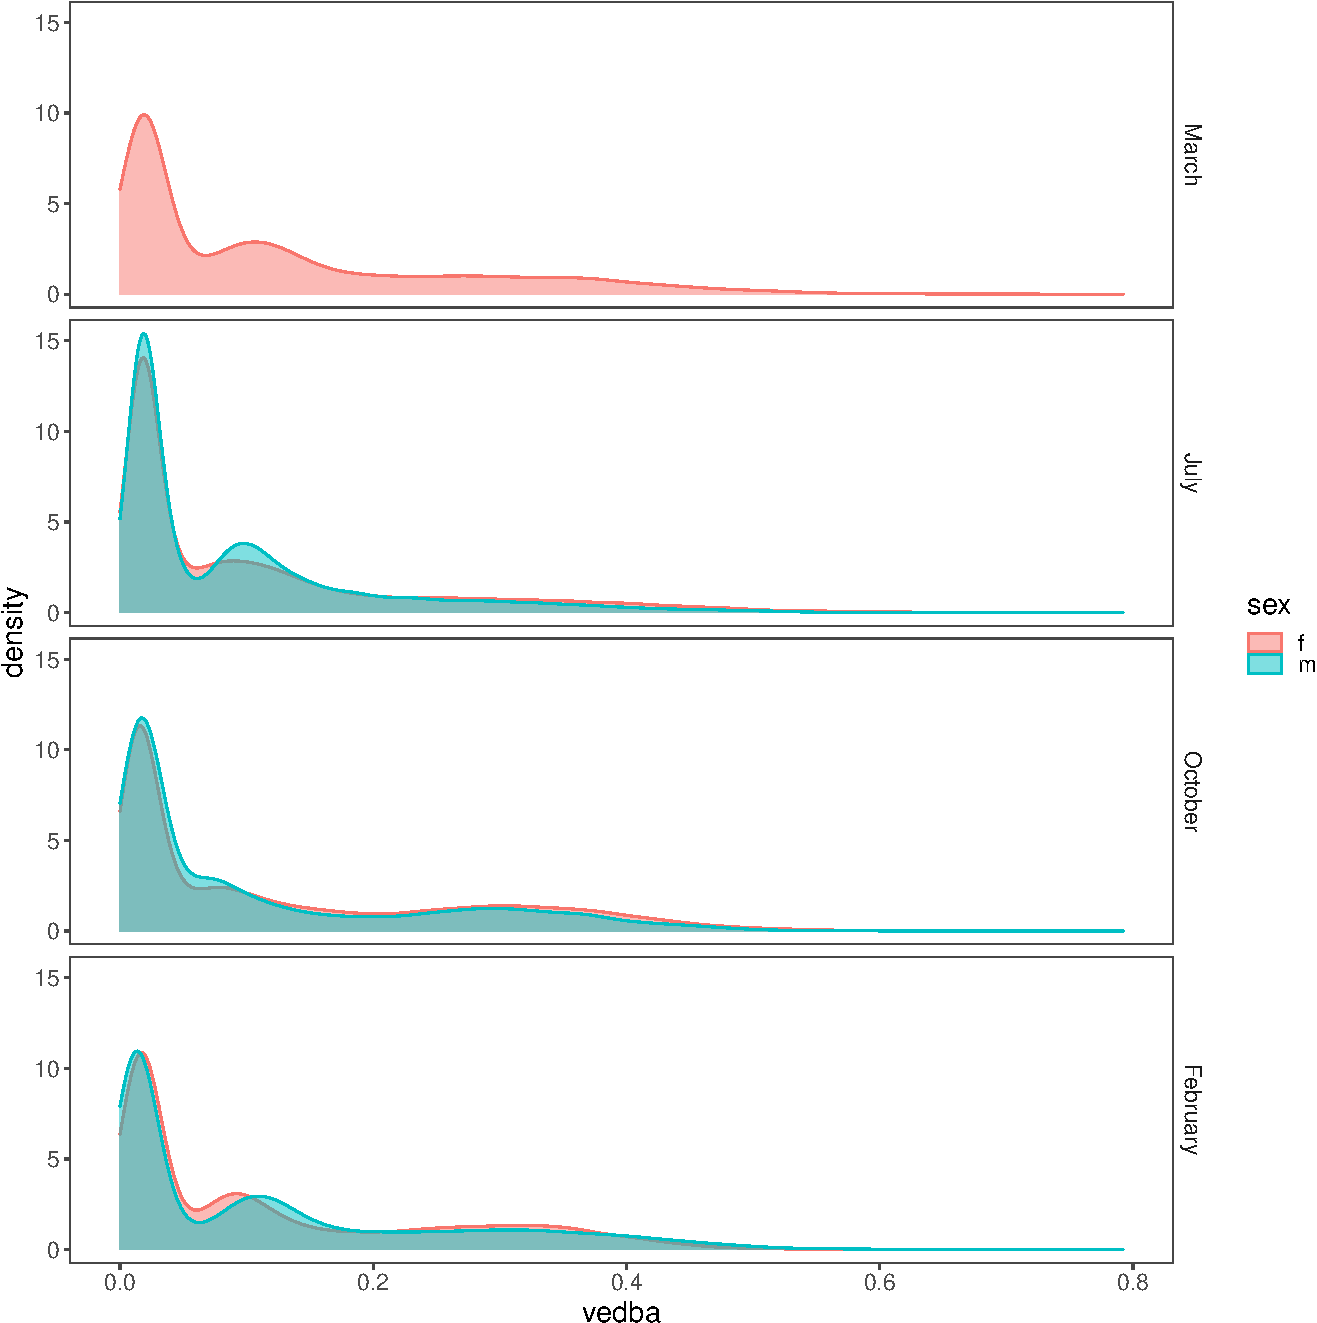
\includegraphics[width=1\linewidth]{tese_jefferson_files/figure-latex/density-season-sex-1} \end{center}

  \newpage

  \hypertarget{medianas-e-boxplots}{%
  \subsection{Medianas e Boxplots}\label{medianas-e-boxplots}}
  \begin{table}[!h]
  \centering
  \begin{tabular}{cccccc}
  \toprule
  season & sex & median & mean & n.animals & n.points\\
  \midrule
  March & f & 0.076 & 0.124 & 2 & 17278\\
  July & f & 0.049 & 0.108 & 5 & 41755\\
  July & m & 0.040 & 0.093 & 3 & 18717\\
  October & f & 0.070 & 0.133 & 5 & 74875\\
  October & m & 0.041 & 0.110 & 1 & 21599\\
  \addlinespace
  February & f & 0.074 & 0.122 & 3 & 33117\\
  February & m & 0.074 & 0.121 & 2 & 28798\\
  \bottomrule
  \end{tabular}
  \end{table}
  \begin{center}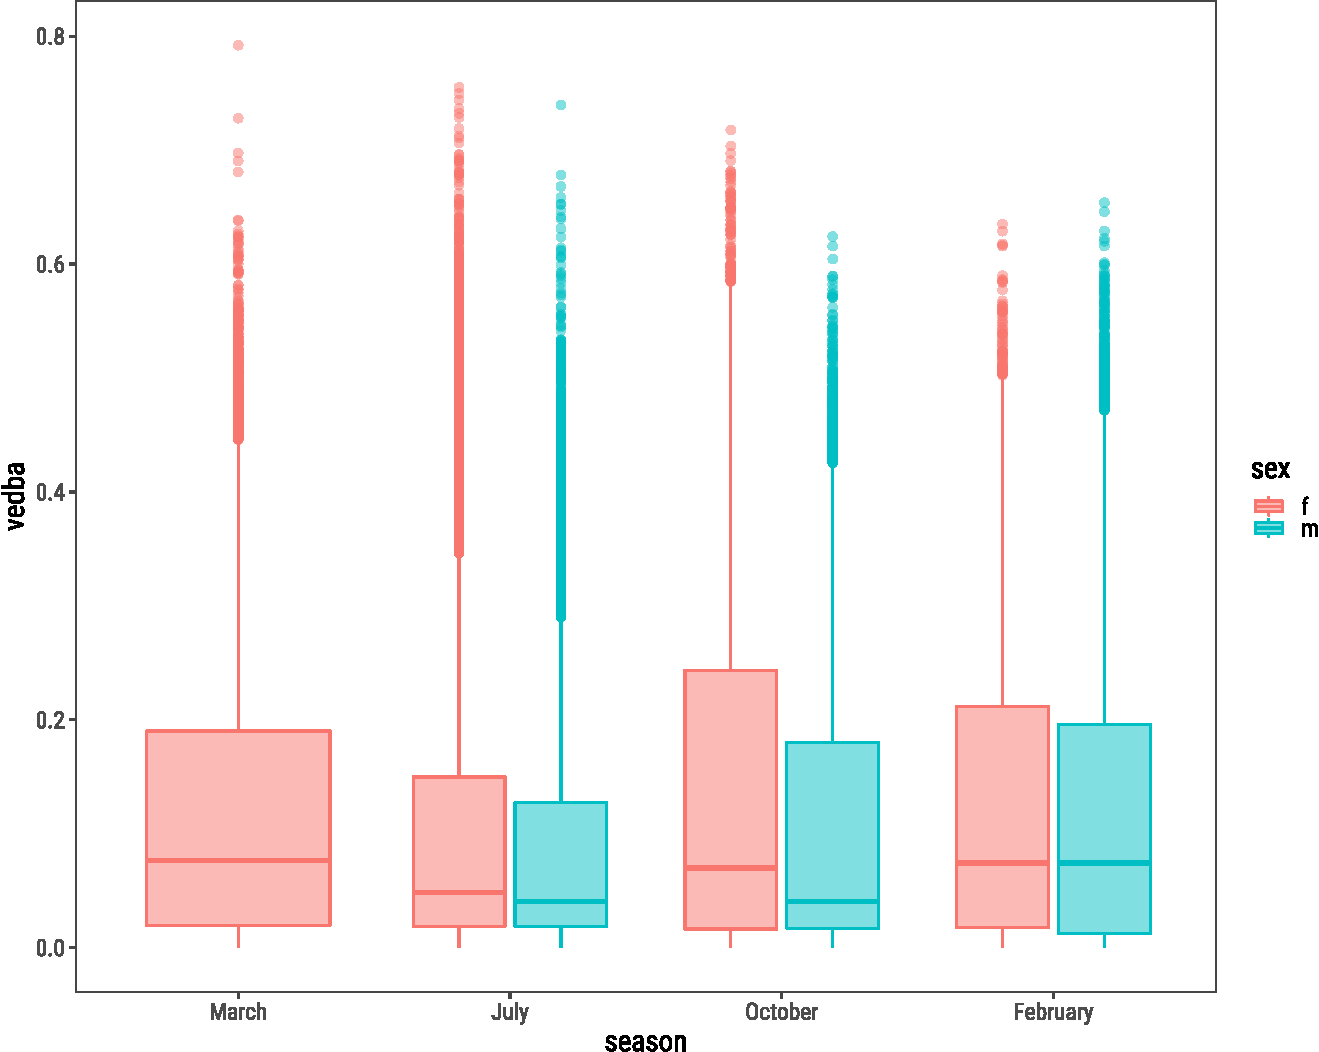
\includegraphics[width=1\linewidth]{tese_jefferson_files/figure-latex/boxplot-season-sex-1} \end{center}

  \hypertarget{ecdf}{%
  \section{ECDF}\label{ecdf}}
  \begin{center}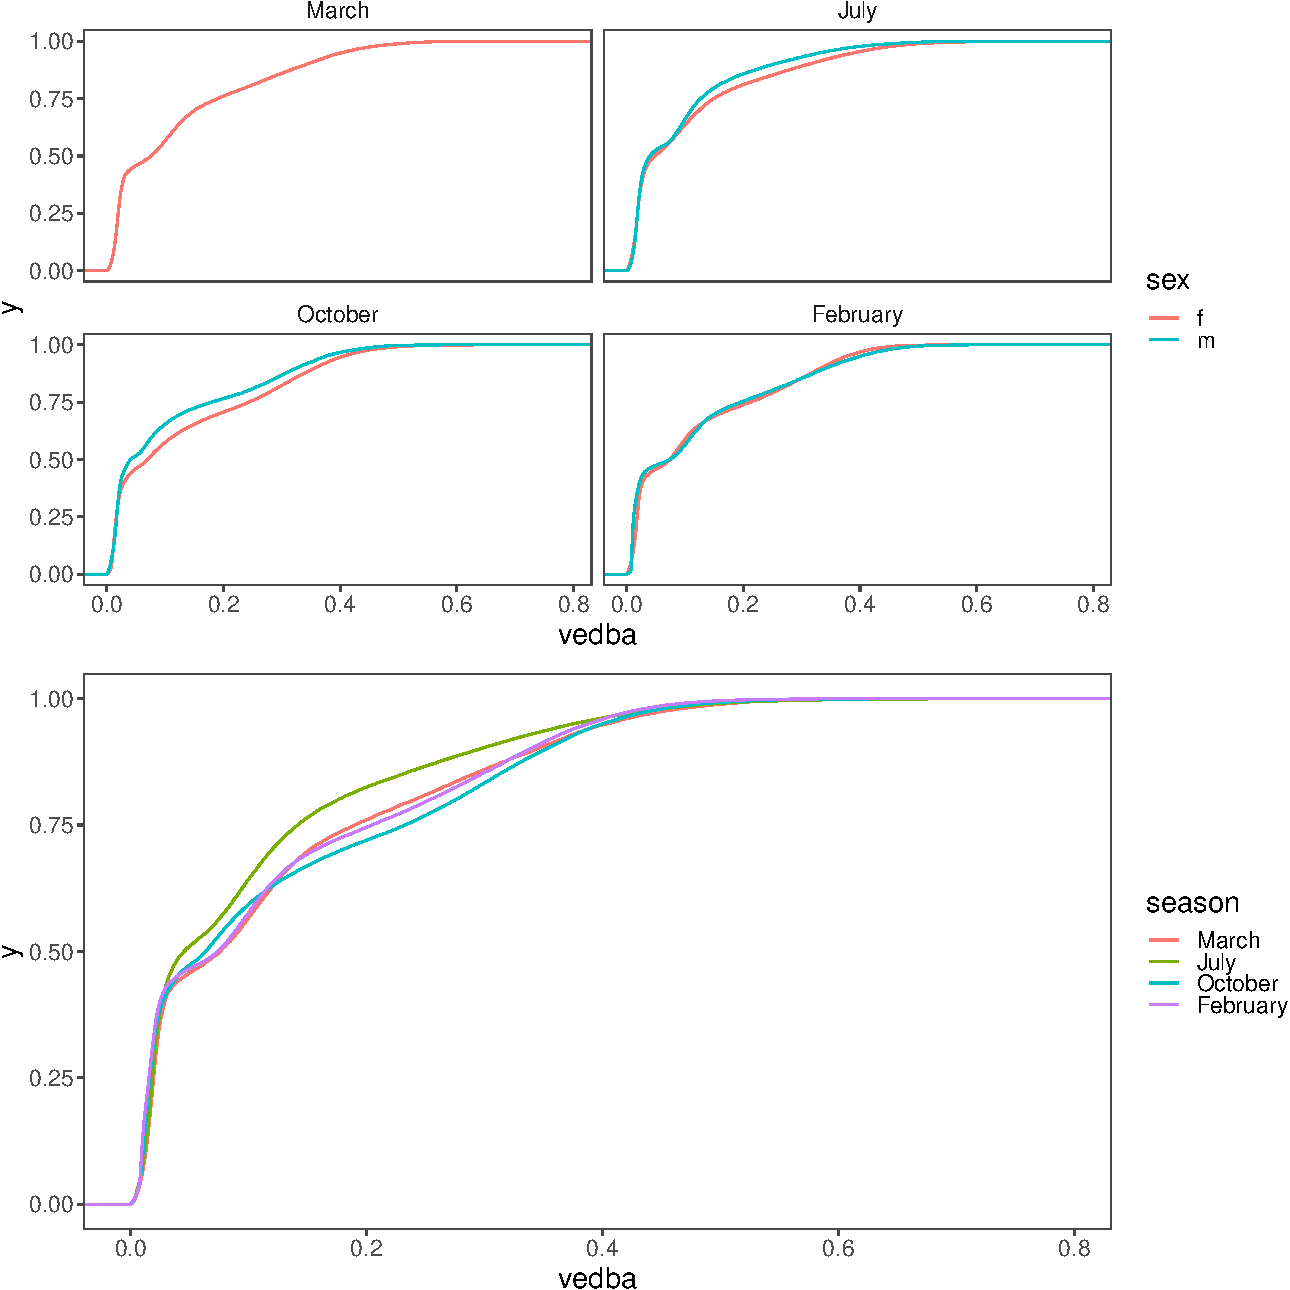
\includegraphics[width=1\linewidth]{tese_jefferson_files/figure-latex/unnamed-chunk-2-1} \end{center}

  \newpage

  \hypertarget{padruxe3o-muxe9dio-de-atividade-por-estauxe7uxe3o-e-sexo}{%
  \section{Padrão Médio de Atividade por Estação e Sexo}\label{padruxe3o-muxe9dio-de-atividade-por-estauxe7uxe3o-e-sexo}}

  Nesse último gráfico eu queria verificar se temporalmente existe alguma diferença entre macho e fêmeas. Cada painel é um grupo entre as opções de combinação de sexo e estação.

  As mesma curvas de VeDBA médio por hora são mostradas em cinza ao fundo, onde cada curva representa um animal diferente. Em cores, colorido por estação, está a média de VeDBA por hora do grupo representado no painel.

  Aparentemente também não existe uma diferença tão grande entre machos e fêmeas quanto aos horário de atividade. Porém, temos um n bem baixo de machos capturados o que torna dificil fazermos uma observação muito concreta.
  \begin{center}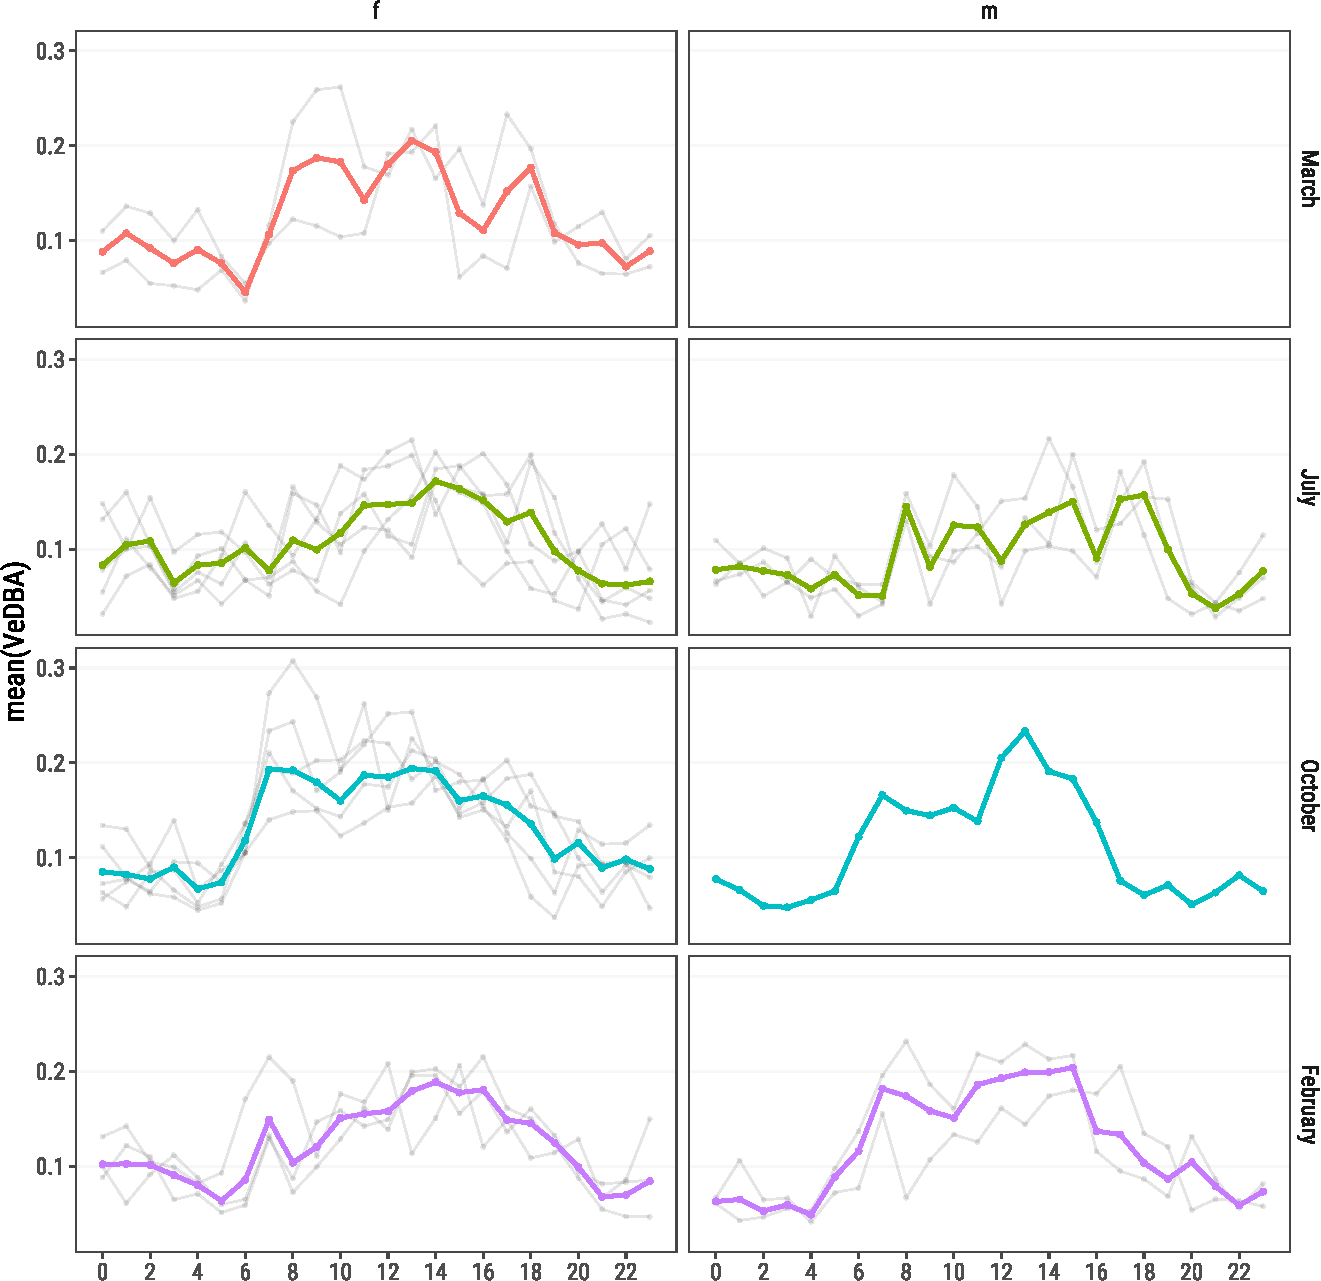
\includegraphics[width=1\linewidth]{tese_jefferson_files/figure-latex/graph-hourly-season-1} \end{center}

  \hypertarget{models-aic}{%
  \chapter{Models' AIC}\label{models-aic}}
  \begin{itemize}
  \tightlist
  \item
    Adicionar o LL
  \end{itemize}
  \begin{table}[!h]
  \centering
  \begin{tabular}{ccc}
  \toprule
  Model & Formula & AIC\\
  \midrule
  m2 & \textasciitilde{}season & -935612.2\\
  m1 & \textasciitilde{}1 & -934800.8\\
  \bottomrule
  \end{tabular}
  \end{table}
  \hypertarget{models-estimated-parameters}{%
  \chapter{Model's Estimated Parameters}\label{models-estimated-parameters}}
  \begin{table}[!h]

  \caption{\label{tab:appendix-parameters}Gamma State-dependent distribution parameters, mean and standard deviation, estimated by a three-state Hidden Markov Model.}
  \centering
  \begin{tabular}[t]{cccc}
  \toprule
  Parameter & State & Estimate & CI\\
  \midrule
  mean & Rest & 0.018 & {}[0.018, 0.018]\\
  mean & Medium & 0.116 & {}[0.116, 0.117]\\
  mean & High & 0.327 & {}[0.326, 0.328]\\
  sd & Rest & 0.010 & {}[0.01, 0.01]\\
  sd & Medium & 0.051 & {}[0.05, 0.051]\\
  \addlinespace
  sd & High & 0.087 & {}[0.086, 0.087]\\
  \bottomrule
  \end{tabular}
  \end{table}
  \hypertarget{pseudo-residuals}{%
  \chapter{Pseudo-residuals}\label{pseudo-residuals}}
  \begin{center}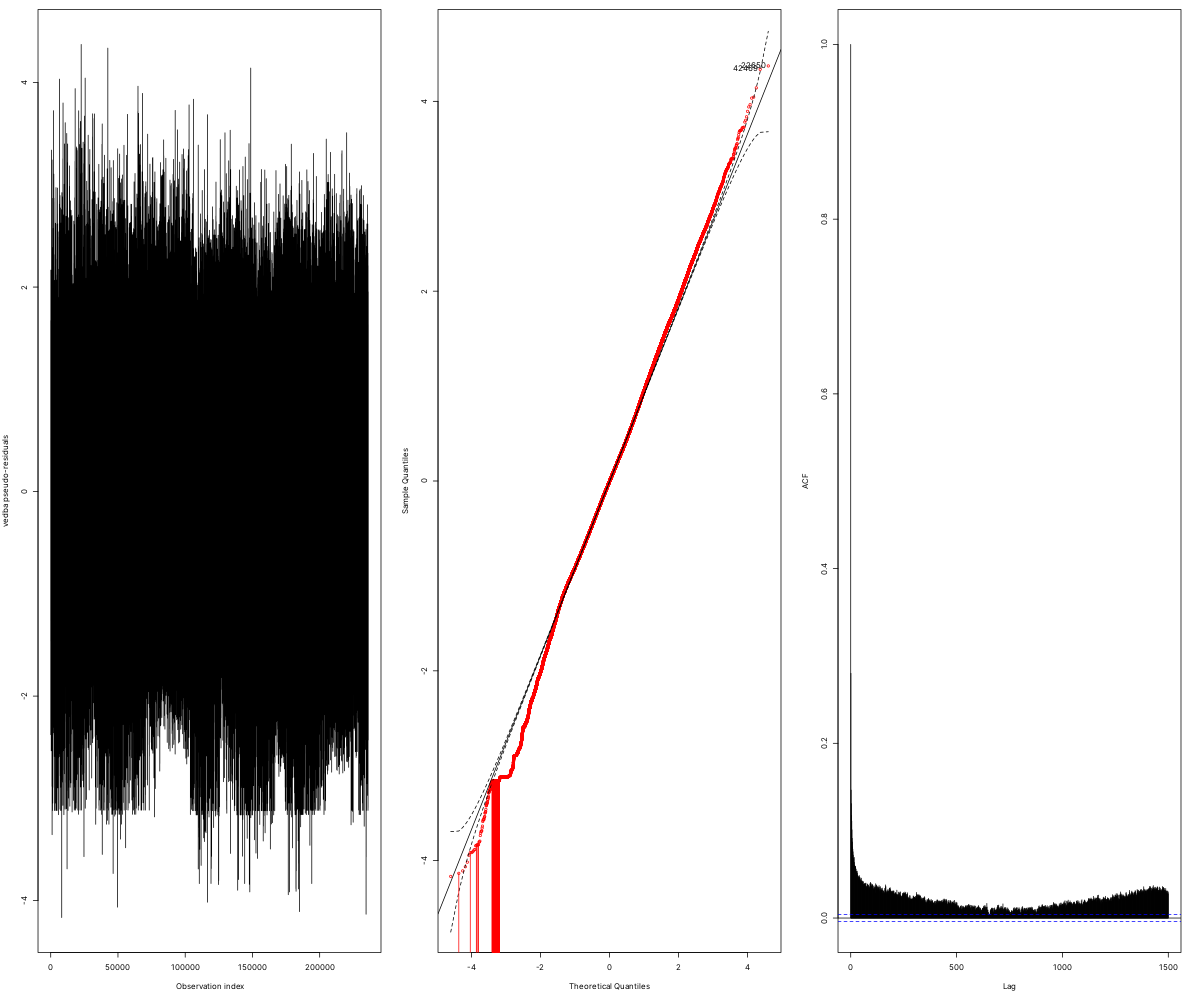
\includegraphics[width=1\linewidth]{../04_figures/residuals/m2_PR} \end{center}

  \hypertarget{vedba-actograms}{%
  \chapter{VeDBA Actograms}\label{vedba-actograms}}
  \begin{center}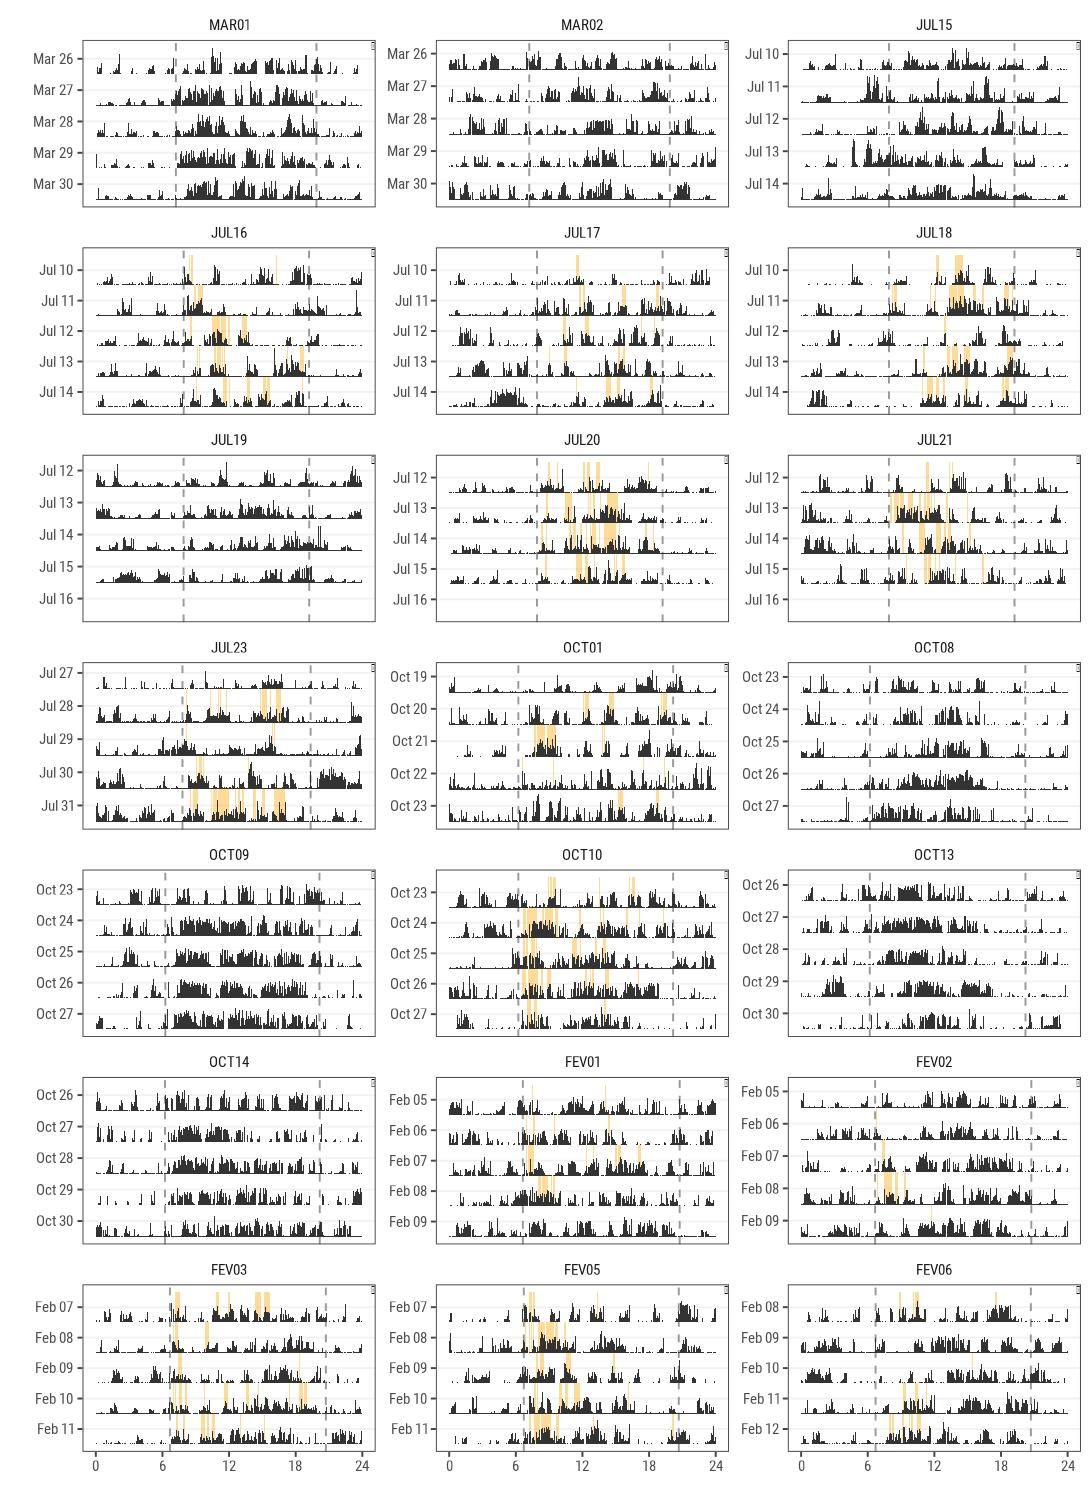
\includegraphics[width=0.95\linewidth]{../04_figures/actograms/actograms_vedba} \end{center}

  \hypertarget{high-activity-actograms}{%
  \chapter{High Activity Actograms}\label{high-activity-actograms}}
  \begin{center}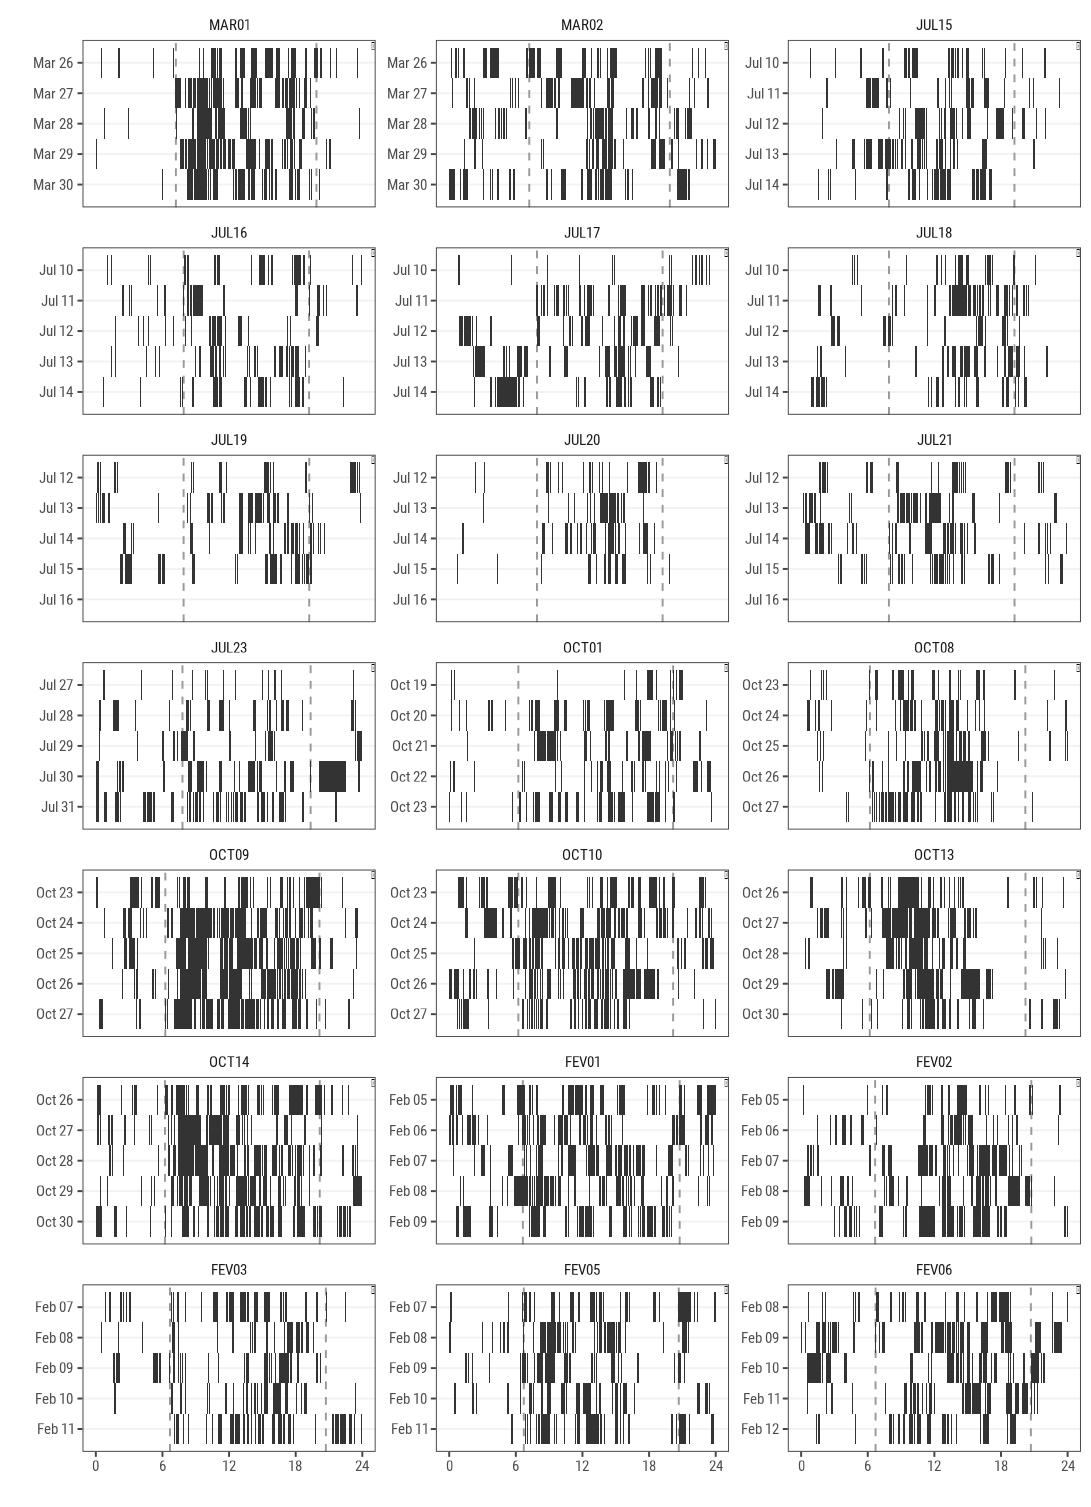
\includegraphics[width=0.95\linewidth]{../04_figures/actograms/actograms_high} \end{center}

  \hypertarget{medium-activity-actograms}{%
  \chapter{Medium Activity Actograms}\label{medium-activity-actograms}}
  \begin{center}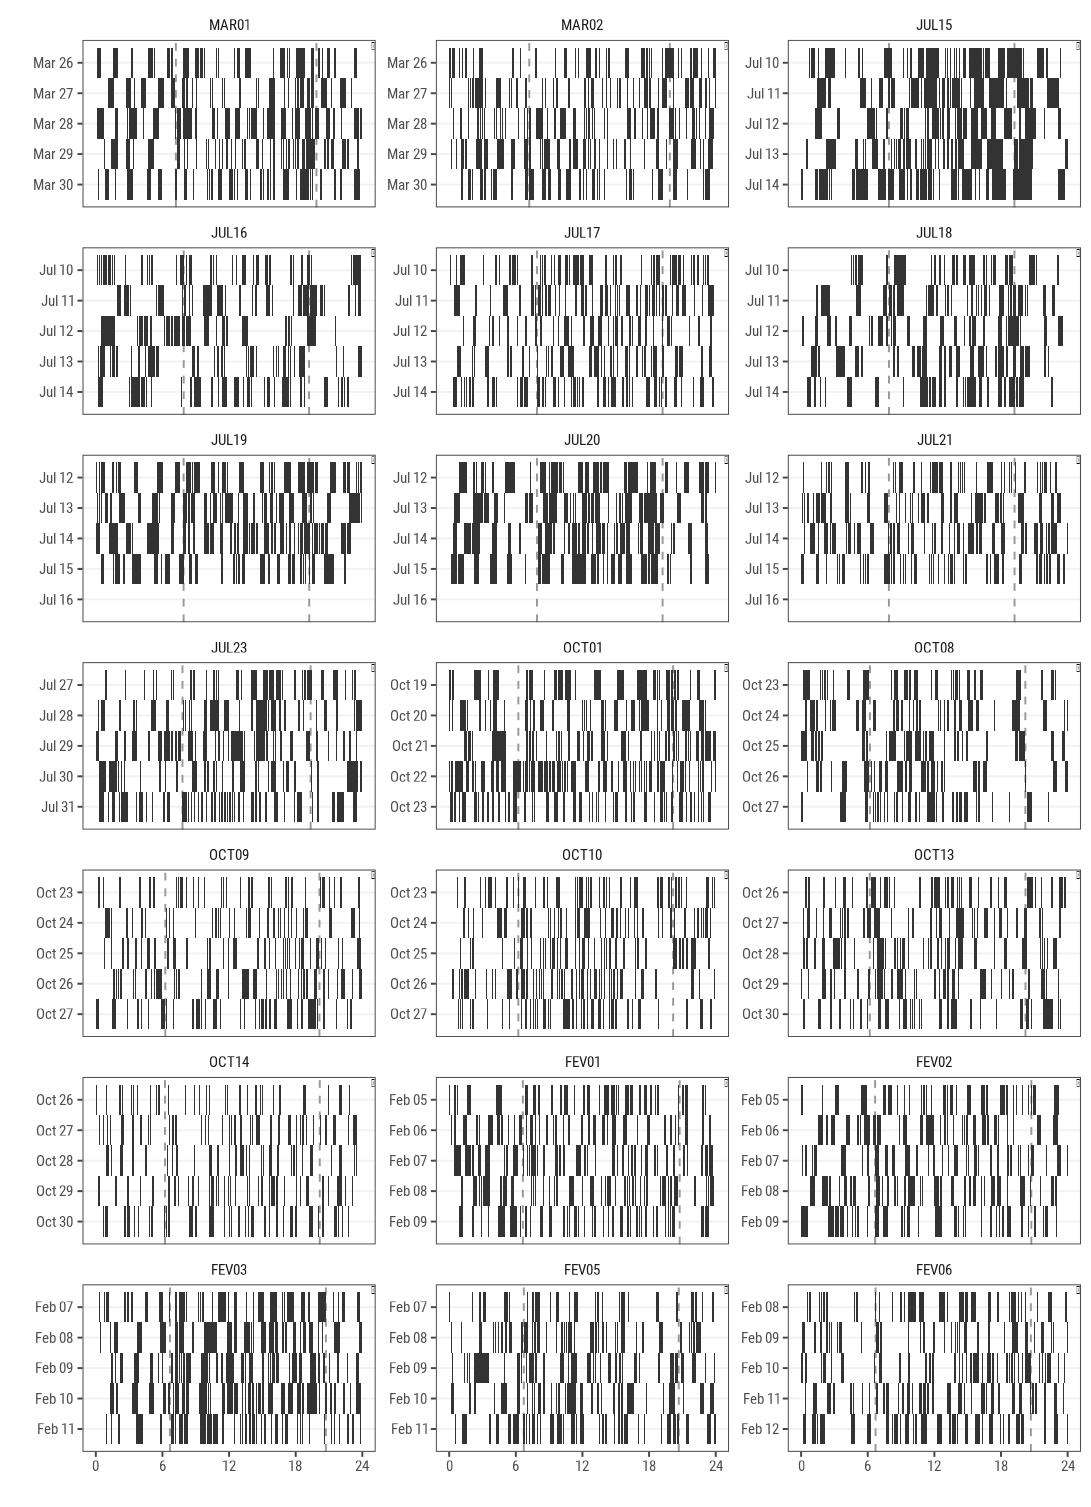
\includegraphics[width=0.95\linewidth]{../04_figures/actograms/actograms_medium} \end{center}

  \hypertarget{medium-activity-daily-patterns}{%
  \chapter{Medium Activity Daily Patterns}\label{medium-activity-daily-patterns}}

  \backmatter
  \bibliographystyle{$biblio-style$}
  \bibliography{thesis}

  \hypertarget{references}{%
  \chapter*{References}\label{references}}
  \addcontentsline{toc}{chapter}{References}

  \noindent

  \setlength{\parindent}{-0.20in}
  \setlength{\leftskip}{0.20in}
  \setlength{\parskip}{8pt}

  \hypertarget{refs}{}
  \begin{CSLReferences}{1}{0}
  \leavevmode\hypertarget{ref-abraham2009}{}%
  Abraham, E., H.F. del Valle, F. Roig, L. Torres, J.O. Ares, F. Coronato, and R. Godagnone. 2009. {``Overview of the Geography of the Monte Desert Biome (Argentina).''} \emph{Journal of Arid Environments} 73 (2): 144--53. \url{https://doi.org/10.1016/j.jaridenv.2008.09.028}.

  \leavevmode\hypertarget{ref-amaya2016}{}%
  Amaya, Juan Pablo, Juan I. Areta, Veronica S. Valentinuzzi, and Emmanuel Zufiaurre. 2016. {``Form and Function of Long-Range Vocalizations in a Neotropical Fossorial Rodent: The Anillaco Tuco-Tuco ( {\emph{Ctenomys}} Sp.).''} \emph{PeerJ} 4 (October): e2559. \url{https://doi.org/10.7717/peerj.2559}.

  \leavevmode\hypertarget{ref-aranda-rickert2014}{}%
  Aranda-Rickert, Adriana, Patricia Diez, and Brigitte Marazzi. 2014. {``Extrafloral Nectar Fuels Ant Life in Deserts.''} \emph{AoB PLANTS} 6 (January). \url{https://doi.org/10.1093/aobpla/plu068}.

  \leavevmode\hypertarget{ref-aranda-rickert2011a}{}%
  Aranda-Rickert, Adriana, and Sebastián Fracchia. 2011. {``Pogonomyrmexcunicularius as the Keystone Disperser of Elaiosome-Bearing Jatropha Excisa Seeds in Semi-Arid Argentina: Pogonomyrmex Cunicularius Ants as Keystone Seed Dispersers.''} \emph{Entomologia Experimentalis Et Applicata} 139 (2): 91--102. \url{https://doi.org/10.1111/j.1570-7458.2011.01111.x}.

  \leavevmode\hypertarget{ref-bivand2020}{}%
  Bivand, Roger, and Nicholas Lewin-Koh. 2020. {``Maptools: Tools for Handling Spatial Objects.''} \url{https://CRAN.R-project.org/package=maptools}.

  \leavevmode\hypertarget{ref-burnham2002}{}%
  Burnham, Kenneth P., David Raymond Anderson, and Kenneth P. Burnham. 2002. \emph{Model Selection and Multimodel Inference: A Practical Information-Theoretic Approach}. 2nd ed. New York: Springer.

  \leavevmode\hypertarget{ref-fracchia2011}{}%
  Fracchia, S., L. Krapovickas, A. Aranda-Rickert, and V.S. Valentinuzzi. 2011. {``Dispersal of Arbuscular Mycorrhizal Fungi and Dark Septate Endophytes by Ctenomys Cf. Knighti (Rodentia) in the Northern Monte Desert of Argentina.''} \emph{Journal of Arid Environments} 75 (11): 1016--23. \url{https://doi.org/10.1016/j.jaridenv.2011.04.034}.

  \leavevmode\hypertarget{ref-jannetti2019}{}%
  Jannetti, Milene G., C. Loren Buck, Veronica S. Valentinuzzi, and Gisele A. Oda. 2019. {``Day and Night in the Subterranean: Measuring Daily Activity Patterns of Subterranean Rodents (Ctenomys Aff. Knighti) Using Bio-Logging.''} \emph{Conservation Physiology} 7 (1). \url{https://doi.org/10.1093/conphys/coz044}.

  \leavevmode\hypertarget{ref-langrock2012}{}%
  Langrock, Roland, Ruth King, Jason Matthiopoulos, Len Thomas, Daniel Fortin, and Juan M. Morales. 2012. {``Flexible and Practical Modeling of Animal Telemetry Data: Hidden Markov Models and Extensions.''} \emph{Ecology} 93 (11): 2336--42. \url{https://doi.org/10.1890/11-2241.1}.

  \leavevmode\hypertarget{ref-leosbarajas2017}{}%
  Leos-Barajas, Vianey, Theoni Photopoulou, Roland Langrock, Toby A. Patterson, Yuuki Y. Watanabe, Megan Murgatroyd, and Yannis P. Papastamatiou. 2017. {``Analysis of Animal Accelerometer Data Using Hidden Markov Models.''} Edited by Robert B. O'Hara. \emph{Methods in Ecology and Evolution} 8 (2): 161--73. \url{https://doi.org/10.1111/2041-210X.12657}.

  \leavevmode\hypertarget{ref-mcclintock2020}{}%
  McClintock, Brett T., Roland Langrock, Olivier Gimenez, Emmanuelle Cam, David L. Borchers, Richard Glennie, and Toby A. Patterson. 2020. {``Uncovering Ecological State Dynamics with Hidden Markov Models.''} Edited by Tim Coulson. \emph{Ecology Letters} 23 (12): 1878--1903. \url{https://doi.org/10.1111/ele.13610}.

  \leavevmode\hypertarget{ref-mcclintock2021}{}%
  McClintock, Brett T, and Theo Michelot. 2021. {``momentuHMM: R Package for Analysis of Telemetry Data Using Generalized Multivariate Hidden Markov Models of Animal Movement,''} 155.

  \leavevmode\hypertarget{ref-michelot2019}{}%
  Michelot, Theo, and Roland Langrock. 2019. {``A Short Guide to Choosing Initial Parameter Values for the Estimation in moveHMM,''} 10.

  \leavevmode\hypertarget{ref-papastamatiou2018}{}%
  Papastamatiou, Yannis P., Yuuki Y. Watanabe, Urška Demšar, Vianey Leos-Barajas, Darcy Bradley, Roland Langrock, Kevin Weng, Christopher G. Lowe, Alan M. Friedlander, and Jennifer E. Caselle. 2018. {``Activity Seascapes Highlight Central Place Foraging Strategies in Marine Predators That Never Stop Swimming.''} \emph{Movement Ecology} 6 (1): 9. \url{https://doi.org/10.1186/s40462-018-0127-3}.

  \leavevmode\hypertarget{ref-patterson2019}{}%
  Patterson, Allison, Hugh Grant Gilchrist, Lorraine Chivers, Scott Hatch, and Kyle Elliott. 2019. {``A Comparison of Techniques for Classifying Behavior from Accelerometers for Two Species of Seabird.''} \emph{Ecology and Evolution} 9 (6): 3030--45. \url{https://doi.org/10.1002/ece3.4740}.

  \leavevmode\hypertarget{ref-patterson2009}{}%
  Patterson, Toby A., Marinelle Basson, Mark V. Bravington, and John S. Gunn. 2009. {``Classifying Movement Behaviour in Relation to Environmental Conditions Using Hidden Markov Models.''} \emph{Journal of Animal Ecology} 78 (6): 1113--23. \url{https://doi.org/10.1111/j.1365-2656.2009.01583.x}.

  \leavevmode\hypertarget{ref-pohle2017}{}%
  Pohle, Jennifer, Roland Langrock, Floris M. van Beest, and Niels Martin Schmidt. 2017. {``Selecting the Number of States in Hidden Markov Models: Pragmatic Solutions Illustrated Using Animal Movement.''} \emph{Journal of Agricultural, Biological and Environmental Statistics} 22 (3): 270--93. \url{https://doi.org/10.1007/s13253-017-0283-8}.

  \leavevmode\hypertarget{ref-qasem2012}{}%
  Qasem, Lama, Antonia Cardew, Alexis Wilson, Iwan Griffiths, Lewis G. Halsey, Emily L. C. Shepard, Adrian C. Gleiss, and Rory Wilson. 2012. {``Tri-Axial Dynamic Acceleration as a Proxy for Animal Energy Expenditure; Should We Be Summing Values or Calculating the Vector?''} \emph{PLOS ONE} 7 (2): e31187. \url{https://doi.org/10.1371/journal.pone.0031187}.

  \leavevmode\hypertarget{ref-rcoreteam2020}{}%
  R Core Team. 2020. {``R: A Language and Environment for Statistical Computing.''} \url{https://www.R-project.org/.}

  \leavevmode\hypertarget{ref-shepard2008}{}%
  Shepard, Elc, Rp Wilson, Lg Halsey, F Quintana, A Gómez Laich, Ac Gleiss, N Liebsch, Ae Myers, and B Norman. 2008. {``Derivation of Body Motion via Appropriate Smoothing of Acceleration Data.''} \emph{Aquatic Biology} 4 (December): 235--41. \url{https://doi.org/10.3354/ab00104}.

  \leavevmode\hypertarget{ref-tomotani2012}{}%
  Tomotani, Barbara M., Danilo E. F. L. Flores, Patrícia Tachinardi, José D. Paliza, Gisele A. Oda, and Verônica S. Valentinuzzi. 2012. {``Field and Laboratory Studies Provide Insights into the Meaning of Day-Time Activity in a Subterranean Rodent (Ctenomys Aff. Knighti), the Tuco-Tuco.''} Edited by Ralph E. Mistlberger. \emph{PLoS ONE} 7 (5): e37918. \url{https://doi.org/10.1371/journal.pone.0037918}.

  \leavevmode\hypertarget{ref-valentinuzzi2009}{}%
  Valentinuzzi, Verónica Sandra, Gisele Akemi Oda, John Fontenele Araújo, and Martin Roland Ralph. 2009. {``Circadian Pattern of Wheel{-}Running Activity of a South American Subterranean Rodent ( {\emph{Ctenomys Cf Knightii}} ).''} \emph{Chronobiology International} 26 (1): 14--27. \url{https://doi.org/10.1080/07420520802686331}.

  \leavevmode\hypertarget{ref-vandekerk2015}{}%
  van de Kerk, Madelon, David P. Onorato, Marc A. Criffield, Benjamin M. Bolker, Ben C. Augustine, Scott A. McKinley, and Madan K. Oli. 2015. {``Hidden Semi-Markov Models Reveal Multiphasic Movement of the Endangered Florida Panther.''} Edited by Tim Coulson. \emph{Journal of Animal Ecology} 84 (2): 576--85. \url{https://doi.org/10.1111/1365-2656.12290}.

  \leavevmode\hypertarget{ref-williams2014}{}%
  Williams, Cory T., Kathryn Wilsterman, Amanda D. Kelley, André R. Breton, Herbert Stark, Murray M. Humphries, Andrew G. McAdam, Brian M. Barnes, Stan Boutin, and C. Loren Buck. 2014. {``Light Loggers Reveal Weather-Driven Changes in the Daily Activity Patterns of Arboreal and Semifossorial Rodents.''} \emph{Journal of Mammalogy} 95 (6): 1230--39. \url{https://doi.org/10.1644/14-MAMM-A-062}.

  \leavevmode\hypertarget{ref-zucchini2016}{}%
  Zucchini, Walter, Iain MacDonald, and Roland Langrock. 2016. \emph{Hidden Markov Models for Time Series - An Introduction Using R}. Vol. 43.

  \end{CSLReferences}
\end{document}
